% FSE 2027 Industry Papers track (companion proceedings, ACM sigconf).
% Double-anonymous review is optional for this track. For an anonymous
% submission, use \documentclass[sigconf,screen,review,anonymous]{acmart}.
\PassOptionsToPackage{table}{xcolor}
\documentclass[sigconf,screen]{acmart}
\usepackage{makecell, multirow, url}
\usepackage{pifont}
\usepackage{xcolor}
\usepackage{graphicx}
\usepackage{amsmath}
\usepackage{algorithm}
\usepackage{algpseudocode}
\usepackage{microtype}
\usepackage{array}
\usepackage{enumitem}
\usepackage{booktabs}
\usepackage{colortbl}
\usepackage{tikz}
\usetikzlibrary{patterns,decorations.pathreplacing,positioning,matrix}
\usepackage{pgfplots}
\usepgfplotslibrary{groupplots}
\pgfplotsset{compat=1.18}

\setlength{\aboverulesep}{0.5pt}
\setlength{\belowrulesep}{0.5pt}
\setlength{\cmidrulekern}{2pt}
\setlength{\emergencystretch}{1em}
\hyphenpenalty=1000
\exhyphenpenalty=1000
\hyphenation{light-weight}

% Companion-proceedings metadata, following the FSE 2026 guidelines;
% confirm against the FSE 2027 Format and Submission Guidelines.
\acmConference[FSE Companion '27]{35th ACM International Conference on the Foundations of Software Engineering}{July 12--16, 2027}{Shenzhen, China}
\acmBooktitle{Companion Proceedings of the 35th ACM International Conference on the Foundations of Software Engineering (FSE Companion '27), July 12--16, 2027, Shenzhen, China}

%%%%% Remove for the final paper
\setcopyright{none} % to remove the copyright notice
\settopmatter{printacmref=false} % to remove the ACM Reference Format
\renewcommand\footnotetextcopyrightpermission[1]{}
%%%%%
\settopmatter{printfolios=true} % page numbers for review

\begin{document}
% Shared macros used by the current camera-framework manuscript.

% Short condition label used in the evaluation tables.
\newcommand{\memory}{{\it mem}}

% Bold upright run-in heading; acmart's \paragraph adds the trailing period.
\newcommand{\myparagraph}[1]{\paragraph{\normalfont\bfseries #1}}

% Fit a tabular to an exact target width by iteratively solving for
% \tabcolsep.  #4 is twice the number of columns.
\newcommand{\fittabcolsepstep}[4]{%
  \sbox{#1}{#2}\addtolength{\tabcolsep}{\dimexpr(#3-\wd#1)/#4\relax}}
\newcommand{\fittabcolsep}[4]{%
  \setlength{\tabcolsep}{0pt}%
  \fittabcolsepstep{#1}{#2}{#3}{#4}\fittabcolsepstep{#1}{#2}{#3}{#4}%
  \fittabcolsepstep{#1}{#2}{#3}{#4}\fittabcolsepstep{#1}{#2}{#3}{#4}%
  \fittabcolsepstep{#1}{#2}{#3}{#4}\fittabcolsepstep{#1}{#2}{#3}{#4}%
  \fittabcolsepstep{#1}{#2}{#3}{#4}\fittabcolsepstep{#1}{#2}{#3}{#4}}


\title[Enabling Multi-Frame Composition in a Camera Draft Pipeline]{Enabling Multi-Frame Composition \\
in a Camera Draft Pipeline: Coordinated Admission \\
and Pacing under Capture Deadlines}

\author{Minhyun Park}
\affiliation{%
  \institution{Samsung Electronics}
  \institution{Sungkyunkwan University}
  \city{Suwon}
  \country{Republic of Korea}}
\email{mhyun2.park@samsung.com}

\author{Sooyoung Cha}
\authornote{Corresponding author.}
\affiliation{%
  \institution{Sungkyunkwan University}
  \city{Suwon}
  \country{Republic of Korea}}
\email{sooyoung.cha@skku.edu}

\begin{abstract}
We present the Budget-Aware Draft Controller, which coordinates optional-stage admission and capture pacing to enable lightweight multi-frame composition in the Samsung Galaxy camera's draft pipeline.
In certain shot modes, the initial draft image stays visible because post-processing for the final image is deferred until the application enters the background.
To improve draft image quality, Samsung deployed single-frame stages in the draft sequence and then implemented a multi-frame composition stage.
The existing static thermal guard omits these optional stages at or above a cutoff to prevent Capture Timeout crashes that block release.
However, under parallel capture, added composition work increased queueing delays at the single draft worker while timeout clocks continued to run, causing timeouts even in runs starting below the cutoff.
Timeout onset also varied with resolution, stage configuration, and memory pressure.
The static cutoff therefore cannot account for differences in draft workload and remaining timeout budgets.
Instead, our controller admits an optional stage only when an empirical upper duration estimate for the remaining sequence fits within the capture's remaining budget.
It also delays the next capture opportunity when projected draft workload threatens the latest queued capture's deadline, limiting backlog growth.
Across 28 evaluated settings on two commercial devices with the guard bypassed, all 280 controller runs completed without timeout.
Only coordinated control completed every ablation run, executing multi-frame composition up to 2.0 times as often as admission alone.
The controller is undergoing release validation for a forthcoming Galaxy flagship line.
\end{abstract}


\maketitle

\section{Introduction}

\label{sec:introduction}

The Samsung Galaxy camera publishes an initial user-visible image, the \emph{draft image}, for each capture and later replaces it with the final image from post-processing.
Samsung refers to the processing stages that produce the draft image as the \emph{draft sequence}.
For certain shot modes, post-processing is deferred until the user switches away from the camera application.
The draft image then remains the user-visible result throughout the foreground session, making its visual quality more important.
In the draft sequence, Samsung has already deployed single-frame stages to narrow the draft--final visual gap and implemented lightweight multi-frame composition to reduce it further.

However, lightweight multi-frame composition has not been deployed on any device because its added processing can violate the \emph{Capture Timeout}, a fixed deadline for each draft image.
A violation crashes the application by design and blocks the release.
The camera must meet this deadline while retaining parallel capture, which shortens shot-to-shot intervals by accepting the next shutter input before the preceding draft image is produced.
Yet draft sequences still execute one at a time on a single draft worker, so later captures may have to wait for earlier draft sequences to finish.
Since each capture's timeout clock starts at request acceptance, added work in an earlier draft sequence can consume queued captures' timeout budgets and cause them to miss their deadlines.

Samsung already uses a static thermal guard to mitigate timeout risk from the deployed single-frame stages.
The guard omits optional stages when configuring the draft sequence at overheat level~4 or higher on a 0--6 scale.
However, in our motivating experiment with the guard bypassed, the capture index of the earliest timeout varied with resolution, memory pressure, and enabled draft stages, even at the same starting overheat level.
The overheat level reflects neither how much timeout budget a capture has left nor how much draft work remains.
Deploying multi-frame composition under parallel capture therefore requires runtime control based on remaining timeout budgets and draft workload.

Such runtime control is constrained: the draft pipeline can neither reject an accepted capture nor preempt a running stage.
Skipping optional stages reduces remaining processing time but cannot recover timeout budget already consumed by queueing.
Delaying the next capture opportunity limits further queue growth to preserve budget for subsequent captures.
These mechanisms correspond to workload control~\cite{approxdet-sensys,timecard-sosp} and arrival control~\cite{seda-sosp,breakwater-osdi}, respectively.
The two controls must be coordinated because decisions to execute or skip optional stages change the draft workload on which arrival control depends.

In this paper, we present the Budget-Aware Draft Controller, which coordinates these two controls to enable lightweight multi-frame composition within per-capture deadlines.
A major challenge is deciding how much time to reserve for draft work: too little risks a Capture Timeout, whereas too much needlessly suppresses optional processing or prolongs shot-to-shot intervals.
To address this, \emph{Remaining-Sequence Admission} uses recent stage overruns to calibrate an empirical upper duration estimate for the entire remaining draft sequence and admits an optional stage when this estimate fits within the capture's remaining timeout budget.
\emph{Capture-Availability Pacing} delays the next capture opportunity when projected draft workload exceeds the remaining timeout budget of the most recently enqueued capture.
Both use a shared duration predictor updated from measured durations in the current camera session, without per-device timing tables.

Across 28 Portrait-mode conditions on two commercial devices, the controller completed all 280 runs without Capture Timeout, whereas uncontrolled execution of all optional stages timed out in 225 of 280 runs.
Lightweight multi-frame composition executed on at least 4.5 of the first five captures per run on average in every condition, including those starting at or above the guard's cutoff.
With production-default 12MP capture under normal memory conditions, pacing did not delay the first five captures at starting overheat levels below 4.
Only the controller with both admission and pacing completed all captures on time in all three ablation conditions, while executing multi-frame composition 1.3--2.0 times as often as admission alone.
The controller is integrated into the product branch and is undergoing release validation for a forthcoming Galaxy flagship line.

\smallskip\noindent\textbf{Contributions.}
\begin{itemize}[leftmargin=1.2em]
  \item We characterize how serialized draft execution under parallel capture creates a cross-capture deadline problem for lightweight multi-frame composition, and why a static thermal guard does not reflect per-capture deadline safety.
  \item We present the Budget-Aware Draft Controller, which coordinates remaining-sequence admission with capture-availability pacing. To our knowledge, this is the first work to combine these controls in production camera software under a hard per-capture deadline.
  \item We evaluate the controller on two commercial devices, examining end-to-end effectiveness, component contribution, admission decision quality against naive approaches, and pacing under queue pressure.
\end{itemize}

\section{Industrial Context and Motivation}
\label{sec:background}

\subsection{Capture Reliability}
\label{sec:release-process}
The Samsung camera software is a privileged system application whose image-capture workflow spans multiple system-level components across the Android software stack.
Consequently, capture failures discovered late in the release cycle may require firmware-level changes involving cross-component coordination and extensive revalidation.
To detect capture failures early, the latest development builds are automatically tested each day across camera workflows, device models, and OS versions.
In addition to this daily testing, the camera-validation team and development engineers periodically stress-test the latest builds to identify timing- and memory-related failures, diagnose their root causes, and verify fixes.
Together, these activities form the core validation process for capture reliability.

\smallskip\noindent\textbf{Capture Timeout.}
A key reliability criterion in this validation process is a fixed internal deadline, referred to as the \emph{Capture Timeout}.
For each capture request, the timeout clock starts at request acceptance, and the ``draft sequence" must produce an initial user-visible draft image before the deadline.
A timeout violation intentionally crashes the application, making the failure immediately observable during testing.
Any such violation blocks the release until developers address its root cause or restrict the affected feature under the conditions that trigger the violation.
Therefore, identifying and resolving Capture Timeout violations is an important reliability task in Samsung's camera development process.

\subsection{Camera Usability}
\label{sec:camera-usability}
\label{sec:draft-background}

The Samsung Galaxy camera must provide high-quality final images and a responsive capture experience.
To improve final image quality, the camera performs post-processing tailored to the camera mode and scene conditions.
This processing typically includes multi-frame composition, which combines complementary information from multiple frames captured for a single shutter input.
For capture responsiveness, the draft sequence provides users with prompt visual feedback before post-processing completes, and parallel capture substantially shortens the shot-to-shot interval by allowing capture requests to overlap.

\myparagraph{Draft sequence}
The draft sequence comprises the processing stages that produce the draft image, which is later replaced by the final image.
The draft image was originally generated from a single captured frame without multi-frame composition.
The draft and final images could therefore differ in appearance, making the replacement noticeable to users.
These differences were particularly pronounced for captures with the Filter or Watermark option enabled, because these effects were applied only to the final image.
To apply these effects to the draft image as well, Samsung added the corresponding single-frame stages to the draft sequence.

% Notes: docs/exhibits.md#fig_draft_final_gap
\begin{figure}[!ht]
  \centering
  \setlength{\tabcolsep}{1pt}%
  % All views are the same 1:1 frame (1080 bp source);
  % the zoom box keeps the source region x 162--702, y 695--875 bp from the bottom.
  % TODO: Replace the middle panel and its crop with the actual draft image
  % produced by lightweight multi-frame composition. Both temporarily reuse
  % fig_draft_final_gap_final.jpg; the caption explicitly marks this placeholder.
  \begin{tabular}{@{}ccc@{}}
    \begin{tikzpicture}
      \node[inner sep=0, anchor=south west] (im) at (0,0)
        {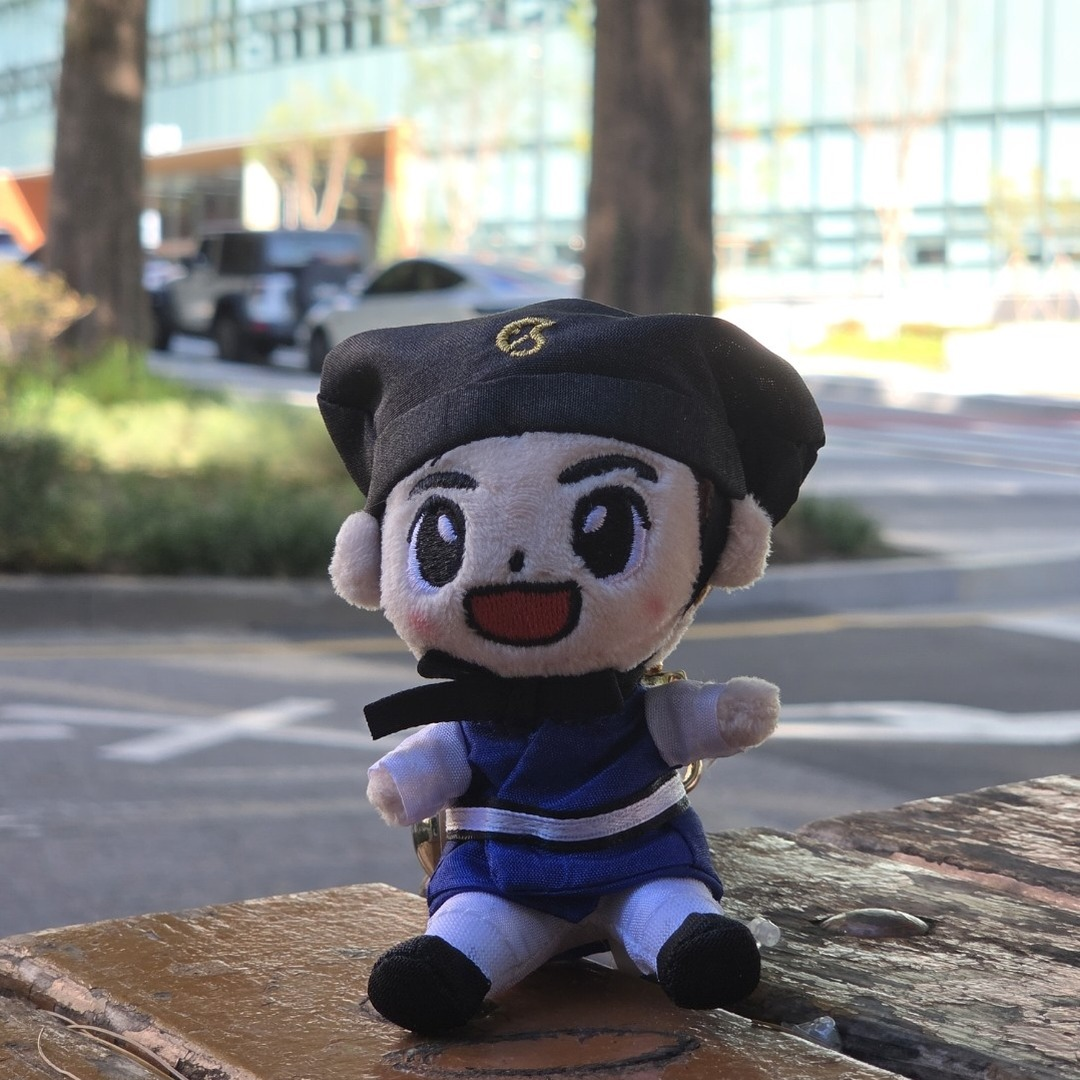
\includegraphics[width=0.325\columnwidth]{figures/fig_draft_final_gap_draft.jpg}};
      \begin{scope}[x={(im.south east)}, y={(im.north west)}]
        \draw[orange, line width=0.8pt] (0.15,0.6435) rectangle (0.65,0.8102);
      \end{scope}
    \end{tikzpicture} &
    \begin{tikzpicture}
      \node[inner sep=0, anchor=south west] (im) at (0,0)
        {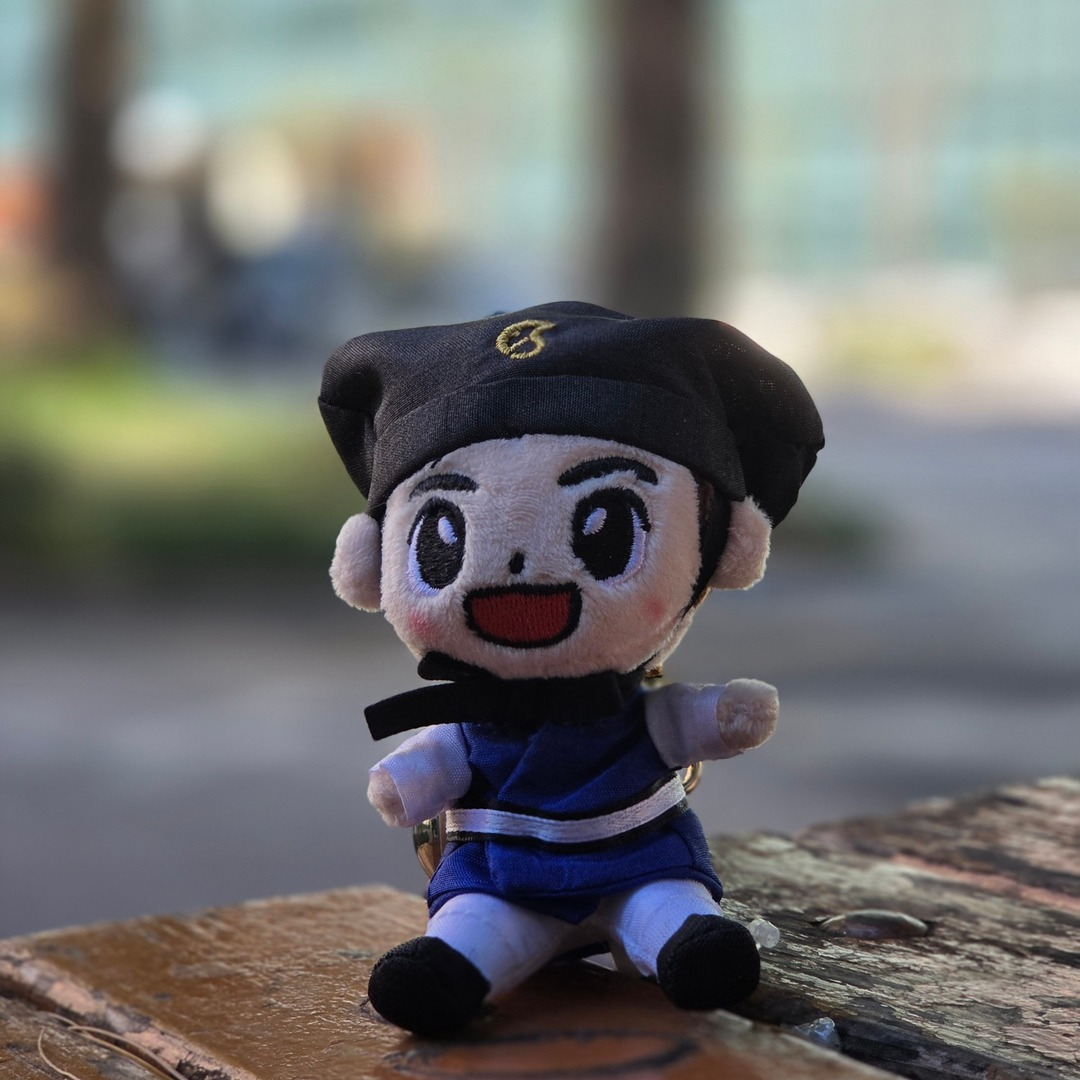
\includegraphics[width=0.325\columnwidth]{figures/fig_draft_final_gap_final.jpg}};
      \begin{scope}[x={(im.south east)}, y={(im.north west)}]
        \draw[orange, line width=0.8pt] (0.15,0.6435) rectangle (0.65,0.8102);
      \end{scope}
    \end{tikzpicture} &
    \begin{tikzpicture}
      \node[inner sep=0, anchor=south west] (im) at (0,0)
        {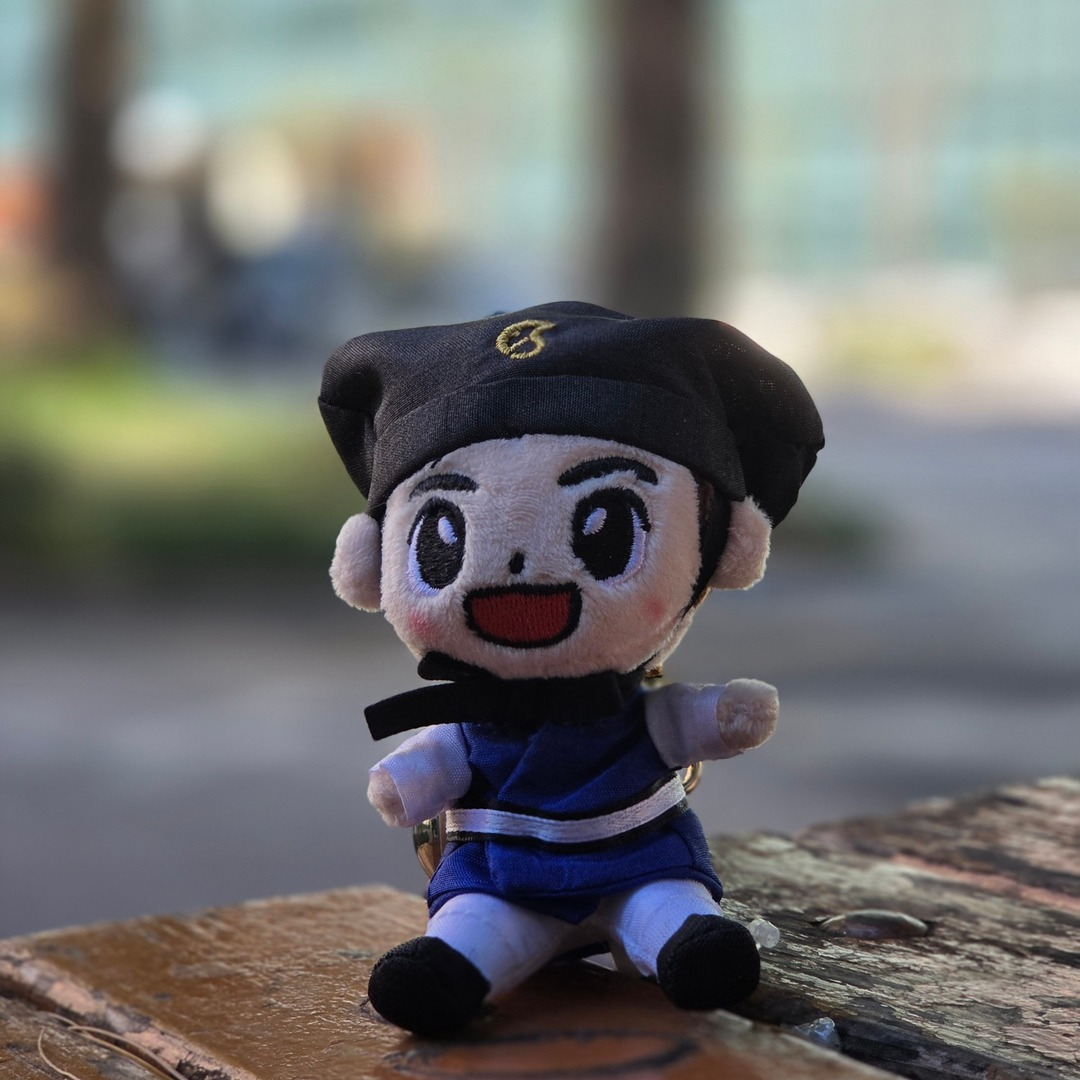
\includegraphics[width=0.325\columnwidth]{figures/fig_draft_final_gap_final.jpg}};
      \begin{scope}[x={(im.south east)}, y={(im.north west)}]
        \draw[orange, line width=0.8pt] (0.15,0.6435) rectangle (0.65,0.8102);
      \end{scope}
    \end{tikzpicture} \tabularnewline[1pt]
    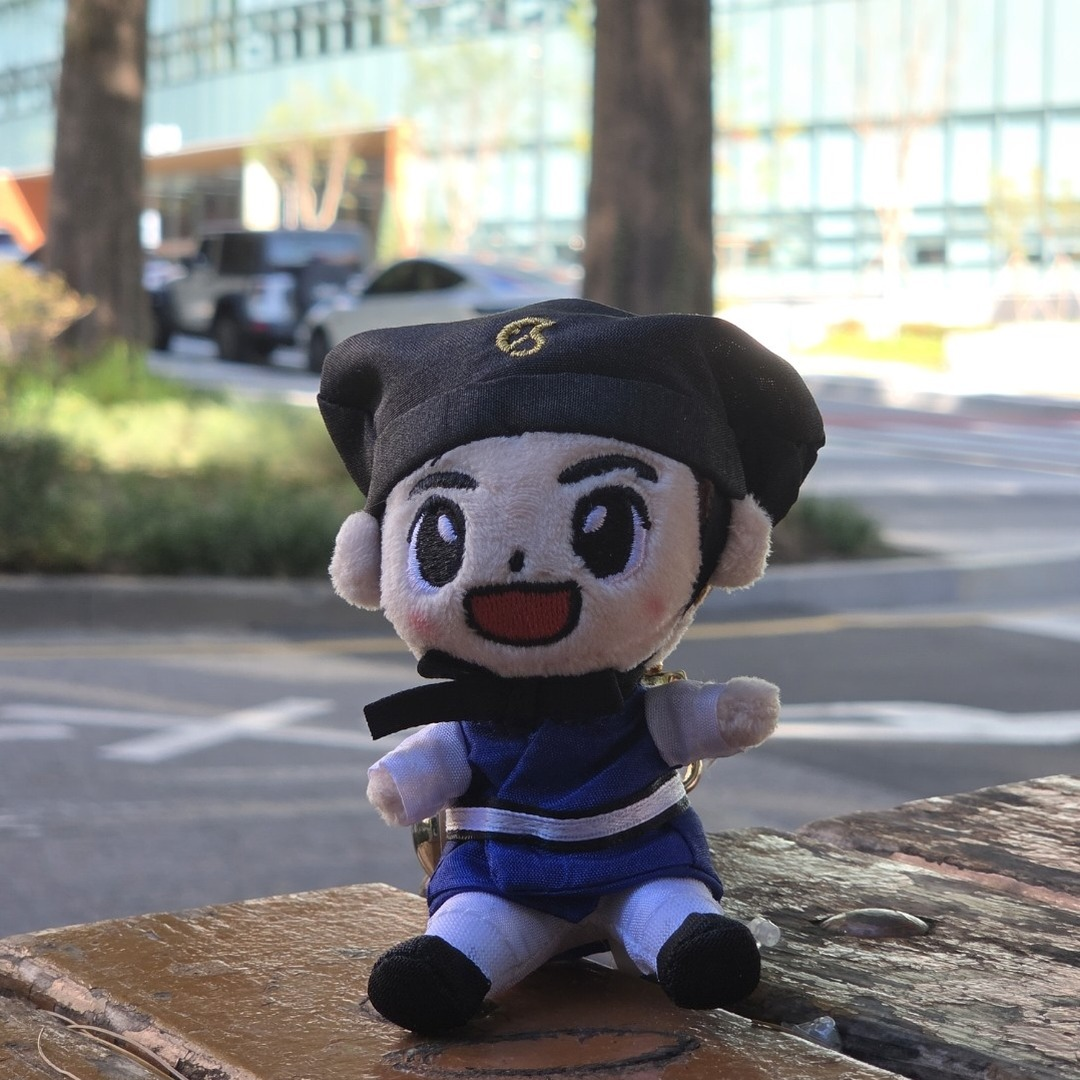
\includegraphics[width=0.325\columnwidth, trim=162 695 378 205, clip]{figures/fig_draft_final_gap_draft.jpg} &
    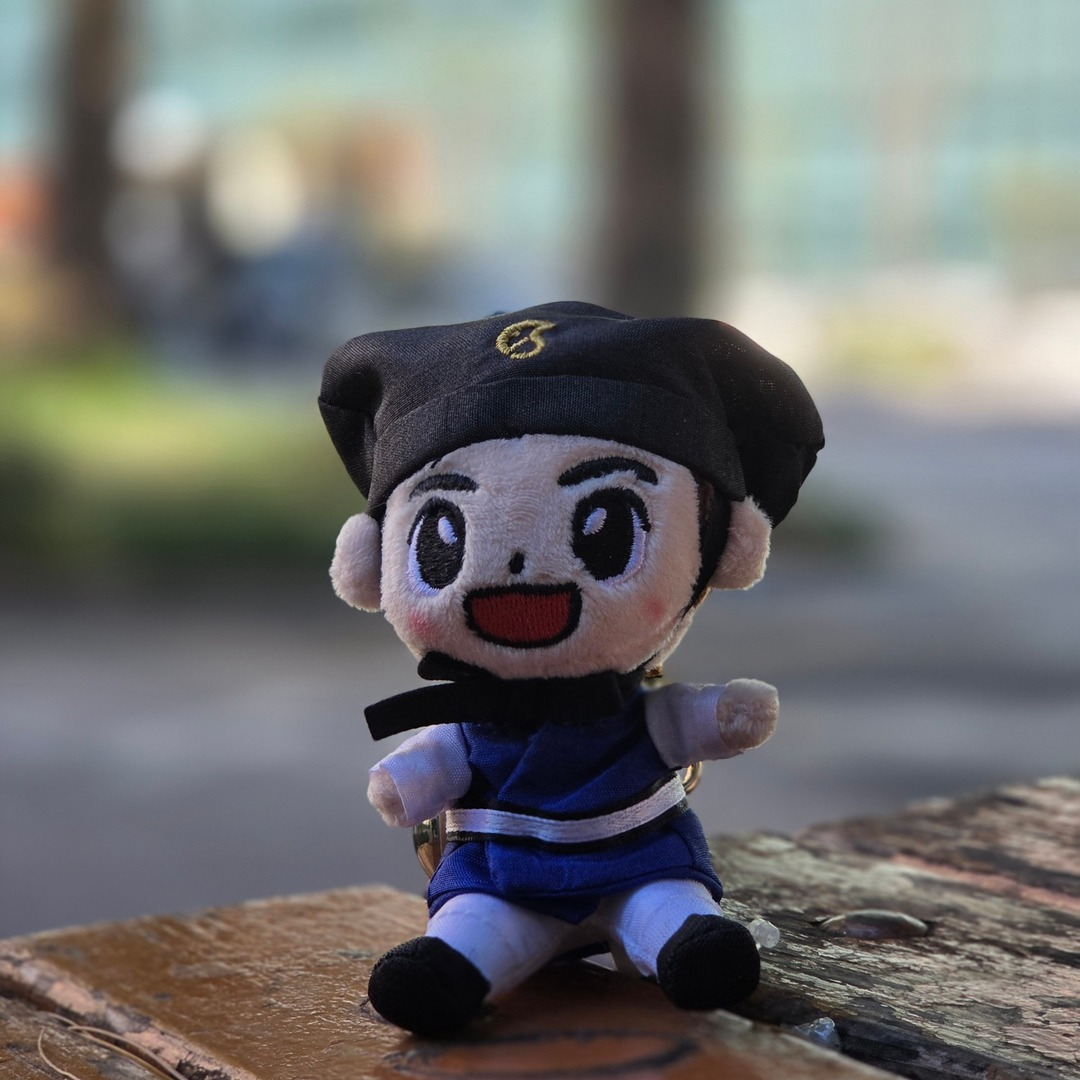
\includegraphics[width=0.325\columnwidth, trim=162 695 378 205, clip]{figures/fig_draft_final_gap_final.jpg} &
    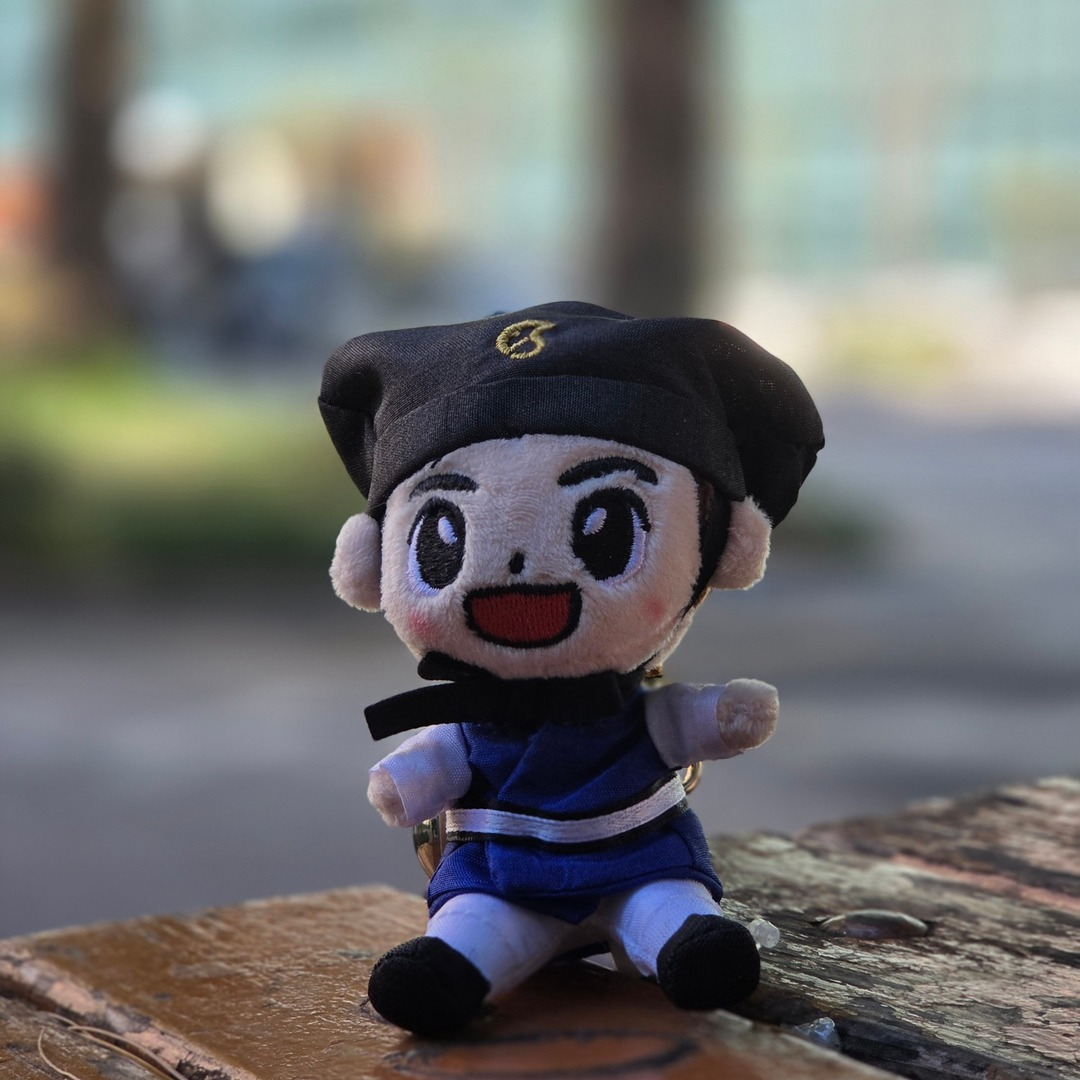
\includegraphics[width=0.325\columnwidth, trim=162 695 378 205, clip]{figures/fig_draft_final_gap_final.jpg}
    \tabularnewline[2pt]
    \parbox[t]{0.325\columnwidth}{\centering\scriptsize (a) Draft image} &
    \makebox[0.325\columnwidth][c]{%
      \parbox[t]{0.41\columnwidth}{\centering\scriptsize
        (b) Draft image with \\lightweight multi-frame composition}} &
    \parbox[t]{0.325\columnwidth}{\centering\scriptsize (c) Final image}
  \end{tabular}
  \caption{Draft--final visual differences in Portrait mode.}
  \label{fig:draft-final-gap}
\end{figure}


As post-processing has advanced over the years and improved final image quality, the visual gap between the draft and final images has continued to widen.
Figure~\ref{fig:draft-final-gap}(a) and~(c) illustrate this gap in Portrait mode.
Post-processing also came to require more computation and resources.
To preserve foreground responsiveness, Samsung deferred the start of post-processing in certain shot modes until the camera application entered the background.
This delays the generation of the final image, so users checking a photo after capture may see the draft image for longer.
Reducing the draft--final visual gap therefore became more important.

To narrow this visual gap, Samsung extended the draft sequence to support a lightweight version of the multi-frame composition used in post-processing.
Figure~\ref{fig:draft-final-gap}(b) shows the draft image produced with lightweight multi-frame composition.
It is closer to the final image in~(c) than the original draft image in~(a), so the replacement is less noticeable.

\myparagraph{Parallel capture}
\label{sec:parallel-capture}
Parallel capture allows the camera application to accept the next shutter input before the preceding capture has produced its draft image.
The camera framework receives a capture-availability signal, \texttt{captureAvailable}, from the hardware abstraction layer (HAL) and forwards it to the application, opening the next capture opportunity.
However, draft sequences execute one at a time on a single draft worker to preserve capture order and limit peak memory demand.
Each draft sequence enters the draft queue after its input frames and metadata have been collected.
Later captures must therefore wait in the draft queue when capture requests arrive faster than the worker completes draft sequences.

\subsection{Capture Timeout Risk}
\label{sec:capture-timeout-risk}
\label{sec:guard-limit}

Enabling lightweight multi-frame composition in the draft sequence increases the risk of a Capture Timeout, especially under parallel capture.
Since each capture's timeout clock starts at request acceptance, waiting in the draft queue consumes part of its timeout budget before its draft sequence starts.
Figure~\ref{fig:overlap} illustrates how this waiting time grows across successive captures even when their draft sequences take equally long.
The additional processing required for lightweight multi-frame composition can lengthen these waits and cause later captures to miss their deadlines.
Because a single Capture Timeout violation blocks release, Samsung has not deployed this feature on any device model.

\begin{figure}[t]
  \centering
  \resizebox{\columnwidth}{!}{% Notes: docs/exhibits.md#fig_parallel_capture_overlap
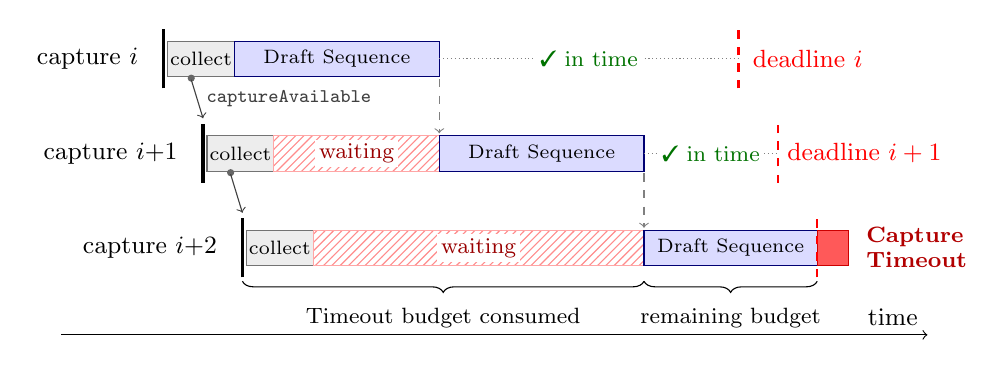
\begin{tikzpicture}[font=\small,
  collectstage/.style={draw=black!55, fill=gray!14},
  draftstage/.style={draw=blue!45!black, fill=blue!14},
  queued/.style={pattern=north east lines, pattern color=red!45, draw=red!35},
  overrun/.style={draw=red!80!black, fill=red!65},
  ddl/.style={red, dashed, thick},
  sig/.style={->, black!75}]

  \node[anchor=east] at (-0.2, 3.925) {capture $i$};
  \draw[very thick] (0, 3.55) -- (0, 4.30);
  \draw[collectstage] (0.05, 3.70) rectangle (0.90, 4.15);
  \node at (0.475, 3.925) {\scriptsize collect};
  \draw[draftstage] (0.90, 3.70) rectangle (3.50, 4.15);
  \node at (2.20, 3.925) {\scriptsize Draft Sequence};

  \draw[densely dotted, gray] (3.50, 3.925) -- (7.30, 3.925);
  \node[fill=white, inner sep=1.5pt] at (5.40, 3.925)
    {\footnotesize\textcolor{green!45!black}{\ding{51} in time}};
  \draw[ddl] (7.30, 3.55) -- (7.30, 4.30);
  \node[red, anchor=east] at (9.00, 3.925) {deadline $i$};

  \fill[black!60] (0.35, 3.68) circle (1.3pt);
  \draw[sig] (0.35, 3.66) -- (0.50, 3.17);
  \node[anchor=west, black!75] at (0.42, 3.42)
    {\scriptsize\texttt{captureAvailable}};

  \node[anchor=east] at (0.3, 2.725) {capture $i{+}1$};
  \draw[very thick] (0.50, 2.35) -- (0.50, 3.10);
  \draw[collectstage] (0.55, 2.50) rectangle (1.40, 2.95);
  \node at (0.975, 2.725) {\scriptsize collect};
  \draw[queued] (1.40, 2.50) rectangle (3.50, 2.95);
  \node[fill=white, inner sep=1.5pt] at (2.45, 2.725)
    {\footnotesize\textcolor{red!60!black}{waiting}};
  \draw[draftstage] (3.50, 2.50) rectangle (6.10, 2.95);
  \node at (4.80, 2.725) {\scriptsize Draft Sequence};

  \draw[densely dotted, gray] (6.10, 2.725) -- (7.80, 2.725);
  \node[fill=white, inner sep=1.5pt] at (6.95, 2.725)
    {\footnotesize\textcolor{green!45!black}{\ding{51} in time}};
  \draw[ddl] (7.80, 2.35) -- (7.80, 3.10);
  \node[red, anchor=east] at (10.00, 2.725) {deadline $i+1$};

  \fill[black!60] (0.85, 2.48) circle (1.3pt);
  \draw[sig] (0.85, 2.46) -- (1.00, 1.97);

  \node[anchor=east] at (0.8, 1.525) {capture $i{+}2$};
  \draw[very thick] (1.00, 1.15) -- (1.00, 1.90);
  \draw[collectstage] (1.05, 1.30) rectangle (1.90, 1.75);
  \node at (1.475, 1.525) {\scriptsize collect};
  \draw[queued] (1.90, 1.30) rectangle (6.10, 1.75);
  \node[fill=white, inner sep=1.5pt] at (4.00, 1.525)
    {\footnotesize\textcolor{red!60!black}{waiting}};
  \draw[draftstage] (6.10, 1.30) rectangle (8.70, 1.75);

  \draw[overrun] (8.30, 1.30) rectangle (8.70, 1.75);
  \node at (7.20, 1.525) {\scriptsize Draft Sequence};
  \draw[ddl] (8.30, 1.15) -- (8.30, 1.90);
  \node[red!70!black, anchor=west, align=left] at (8.80, 1.525)
    {\footnotesize\bfseries Capture\\[-2pt]\footnotesize\bfseries Timeout};

  \draw[dashed, gray, ->] (3.50, 3.67) -- (3.50, 2.98);
  \draw[dashed, gray, ->] (6.10, 2.47) -- (6.10, 1.78);

  \draw[decorate, decoration={brace, mirror, amplitude=4pt}]
    (1.00, 1.10) -- (6.10, 1.10);
  \node[anchor=north] at (3.55, 0.88) {\footnotesize Timeout budget consumed};
  \draw[decorate, decoration={brace, mirror, amplitude=4pt}]
    (6.10, 1.10) -- (8.30, 1.10);
  \node[anchor=north] at (7.20, 0.88) {\footnotesize remaining budget};

  \draw[->] (-1.3, 0.42) -- (9.7, 0.42) node[anchor=south east] {time};

\end{tikzpicture}
}
  \caption{Timeout budget consumed under parallel capture.}
  \label{fig:overlap}
\end{figure}

\myparagraph{Existing thermal guard}
Samsung uses a static thermal guard to prevent Capture Timeout violations in deployed single-frame draft stages.
The guard uses Samsung's overheat level, an ordinal thermal indicator on a 0--6 scale, where larger values denote stronger throttling.
During pre-release validation, throttling at level~4 or higher repeatedly delayed draft sequences and caused Capture Timeout violations despite optimization.
The guard therefore skips optional single-frame stages at these levels.
However, the overheat level does not indicate a capture's waiting time or remaining draft work.
The guard therefore cannot directly assess whether the remaining timeout budget is sufficient for that work.

\myparagraph{Motivating experiment}
To examine the timeout risk of enabling lightweight multi-frame composition in the draft sequence, we compared two Portrait configurations on the Galaxy S26 Ultra.
We bypassed the thermal guard so that configured optional stages could execute regardless of the overheat level.
The optional stages are the multi-frame composition stage (\(M\)) and the deployed single-frame stages (collectively \(S\)).
Both \(M\) alone and \(M+S\) retain the same mandatory encoding and saving stages.
We tested 12MP and 24MP capture under normal memory conditions and under memory pressure.
For each condition in Table~\ref{tab:timeout_index}, we ran ten trials of up to 30 consecutive captures.
We chose 30 captures to extend testing beyond the earlier level-4 validation failure near the 20th consecutive capture.
The table reports the earliest timeout capture index across the ten trials, grouped by starting overheat level.

% Notes: docs/exhibits.md#tab_timeout_index
\providecolor{tmoS1}{RGB}{252,227,220} %
\providecolor{tmoS2}{RGB}{239,160,140} %
\providecolor{tmoS3}{RGB}{201,80,63}  %
\providecolor{tmoS4}{RGB}{143,36,32}  %

\newcolumntype{H}{>{\centering\arraybackslash}m{1.20cm}}
\newcolumntype{P}{>{\centering\arraybackslash}m{0.67cm}}

\providecommand{\tmoFirst}[2]{\cellcolor{#1}\makebox[\linewidth][r]{#2\hspace{1pt}}}
\providecommand{\tmoFirstW}[2]{\cellcolor{#1}\makebox[\linewidth][r]{\textcolor{white}{\textbf{#2}}\hspace{1pt}}}
\providecommand{\tmoNone}{\makebox[\linewidth][r]{--\hspace{1pt}}}

\begin{table}[t]
 \centering
 \caption{Capture index of the earliest timeout.}
 \label{tab:timeout_index}
 {\scriptsize\setlength{\tabcolsep}{1.3pt}%
 \begin{tabular}{@{}HPP|PP||PP|PP@{}}
 \toprule
 \multirow[c]{3}{=}[-10pt]{\makecell[c]{\textbf{Starting}\\\textbf{overheat}\\\textbf{level}}} &
 \multicolumn{4}{c||}{\raisebox{-3pt}{\textbf{Normal capture}}} &
 \multicolumn{4}{c@{}}{\raisebox{-3pt}{\textbf{Memory-pressure capture}}} \\[6pt] \cmidrule(lr){2-5}\cmidrule(l){6-9}
 &
 \multicolumn{2}{c|}{\raisebox{-3pt}{\textbf{12MP}}} &
 \multicolumn{2}{c||}{\raisebox{-3pt}{\textbf{24MP}}} &
 \multicolumn{2}{c|}{\raisebox{-3pt}{\textbf{12MP}}} &
 \multicolumn{2}{c@{}}{\raisebox{-3pt}{\textbf{24MP}}} \\[6pt] \cmidrule(lr){2-3}\cmidrule(lr){4-5}\cmidrule(lr){6-7}\cmidrule(l){8-9}
 & \raisebox{-2pt}{\textbf{M{+}S}} & \raisebox{-2pt}{\textbf{M}} &
 \raisebox{-2pt}{\textbf{M{+}S}} & \raisebox{-2pt}{\textbf{M}} &
 \raisebox{-2pt}{\textbf{M{+}S}} & \raisebox{-2pt}{\textbf{M}} &
 \raisebox{-2pt}{\textbf{M{+}S}} & \raisebox{-2pt}{\textbf{M}} \\[4pt]
 \midrule
 Lv0 &
 \tmoNone & \tmoNone & \tmoFirst{tmoS1}{29} & \tmoNone &
 \tmoNone & \tmoNone & \tmoFirst{tmoS1}{26} & \tmoNone \\
 Lv1 &
 \tmoNone & \tmoNone & \tmoFirst{tmoS1}{29} & \tmoNone &
 \tmoFirst{tmoS1}{24} & \tmoNone & \tmoFirst{tmoS2}{19} & \tmoNone \\
 Lv2 &
 \tmoFirst{tmoS1}{24} & \tmoNone & \tmoFirst{tmoS2}{18} & \tmoNone &
 \tmoFirst{tmoS2}{15} & \tmoFirst{tmoS1}{29} &
 \tmoFirst{tmoS2}{14} & \tmoFirst{tmoS1}{25} \\
 Lv3 &
 \tmoFirst{tmoS2}{13} & \tmoFirst{tmoS1}{21} &
 \tmoFirst{tmoS2}{12} & \tmoFirst{tmoS1}{20} &
 \tmoFirstW{tmoS3}{8} & \tmoFirst{tmoS2}{19} &
 \tmoFirstW{tmoS4}{5} & \tmoFirst{tmoS2}{13} \\
 \midrule
 Lv4 &
 \tmoFirstW{tmoS3}{8} & \tmoFirst{tmoS2}{16} &
 \tmoFirstW{tmoS3}{7} & \tmoFirst{tmoS2}{13} &
 \tmoFirstW{tmoS3}{6} & \tmoFirst{tmoS2}{13} &
 \tmoFirstW{tmoS4}{3} & \tmoFirstW{tmoS3}{7} \\
 Lv5 &
 \tmoFirstW{tmoS3}{8} & \tmoFirst{tmoS2}{12} &
 \tmoFirstW{tmoS3}{8} & \tmoFirst{tmoS2}{12} &
 \tmoFirstW{tmoS4}{4} & \tmoFirstW{tmoS3}{9} &
 \tmoFirstW{tmoS4}{4} & \tmoFirstW{tmoS3}{9} \\
 Lv6 &
 \tmoFirstW{tmoS3}{7} & \tmoFirst{tmoS2}{11} &
 \tmoFirstW{tmoS3}{7} & \tmoFirst{tmoS2}{11} &
 \tmoFirstW{tmoS4}{3} & \tmoFirstW{tmoS3}{6} &
 \tmoFirstW{tmoS4}{3} & \tmoFirstW{tmoS3}{6} \\
 \bottomrule
 \end{tabular}%
 }
 \par\vspace{3pt}
 {\scriptsize\begin{minipage}{0.933\columnwidth}
 \raggedright\setlength{\fboxsep}{1.8pt}%
 Timeout capture index:~%
 \colorbox{tmoS1}{\strut\,${\geq}\,20$\,}\colorbox{tmoS2}{\strut\,10--19\,}\colorbox{tmoS3}{\strut\,\textcolor{white}{6--9}\,}\colorbox{tmoS4}{\strut\,\textcolor{white}{${\leq}\,5$}\,}\par
 --: no timeout observed within 30 captures.\par
 \end{minipage}}
\end{table}


With the thermal guard bypassed, \(M+S\) timed out in 13 of the 16 conditions with starting levels below the guard's cutoff.
Every \(M+S\) trial starting at level~4 or higher nevertheless completed its first capture without a timeout, even though the guard would have skipped the optional stages for that capture.
Even at the same starting level, the earliest timeout varied with resolution, memory pressure, and draft configuration.
In conditions where \(M+S\) timed out, reducing optional work to \(M\) alone delayed the earliest timeout or resulted in no observed timeout within 30 captures.
Together, these observations motivate runtime control of optional-stage execution based on each capture's remaining timeout budget and draft workload, rather than the overheat level alone.
\subsection{Goal}
\label{sec:research-goal}

Our goal is to enable multi-frame composition in the draft sequence under parallel capture to narrow the draft--final visual gap while completing each capture before its Capture Timeout deadline.
Meeting this goal requires controlling both optional draft work and capture arrivals.
Skipping optional stages can reduce processing time but cannot recover timeout budget already spent waiting.
Delaying the next capture opportunity can limit draft queue growth and preserve budget for optional processing.
To determine how much timeout budget to reserve, both decisions require estimating the time needed for the remaining draft work.
Reserving too little time risks a Capture Timeout, whereas reserving too much needlessly sacrifices draft image quality or capture responsiveness.

% \subsection{Draft Sequence}
\label{sec:draft-background}

For each capture, the Samsung camera publishes an initial user-visible draft image through the draft sequence, while the post-processing pipeline produces the final image.
When post-processing completes, the final image replaces the draft image if one has been published.
To preserve capture order and limit peak compute and memory demand, the current pipeline executes draft sequences one at a time on a single draft worker.

As post-processing became more resource-intensive, its start was deferred for certain shot modes until the application entered the background to preserve foreground responsiveness.
In these modes, the draft image remains the user-visible result throughout the foreground session, making its visual quality more important.

Yet the original draft sequence saved an image without additional image processing, and advances in post-processing widened the visual gap between draft and final images.
This draft--final visual gap is particularly pronounced in Super-resolution, Night, High-resolution, and Portrait modes, and Figure~\ref{fig:draft-final-gap}(a) and~(c) show an example from Portrait mode.

% Notes: docs/exhibits.md#fig_draft_final_gap
\begin{figure}[!ht]
  \centering
  \setlength{\tabcolsep}{1pt}%
  % All views are the same 1:1 frame (1080 bp source);
  % the zoom box keeps the source region x 162--702, y 695--875 bp from the bottom.
  % TODO: Replace the middle panel and its crop with the actual draft image
  % produced by lightweight multi-frame composition. Both temporarily reuse
  % fig_draft_final_gap_final.jpg; the caption explicitly marks this placeholder.
  \begin{tabular}{@{}ccc@{}}
    \begin{tikzpicture}
      \node[inner sep=0, anchor=south west] (im) at (0,0)
        {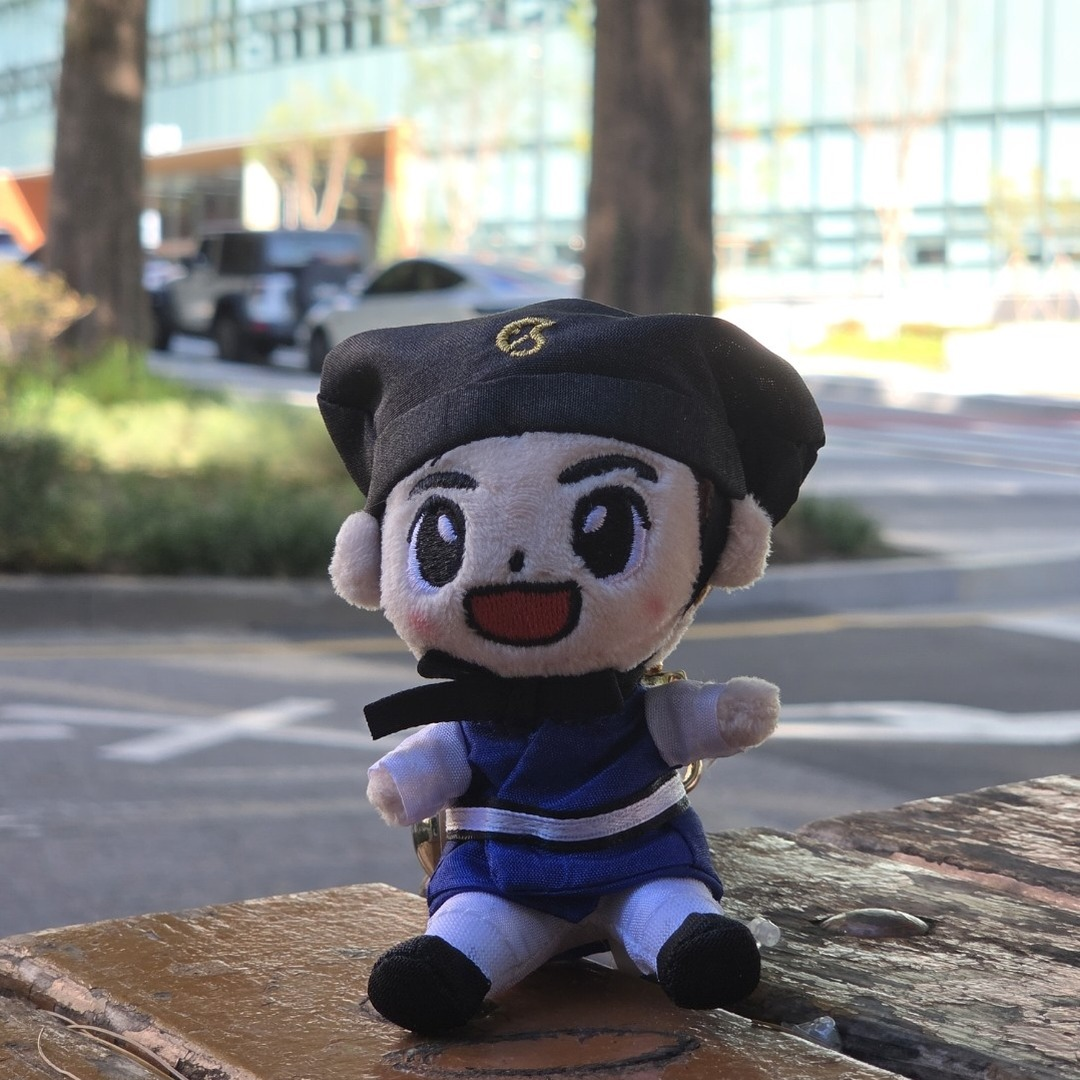
\includegraphics[width=0.325\columnwidth]{figures/fig_draft_final_gap_draft.jpg}};
      \begin{scope}[x={(im.south east)}, y={(im.north west)}]
        \draw[orange, line width=0.8pt] (0.15,0.6435) rectangle (0.65,0.8102);
      \end{scope}
    \end{tikzpicture} &
    \begin{tikzpicture}
      \node[inner sep=0, anchor=south west] (im) at (0,0)
        {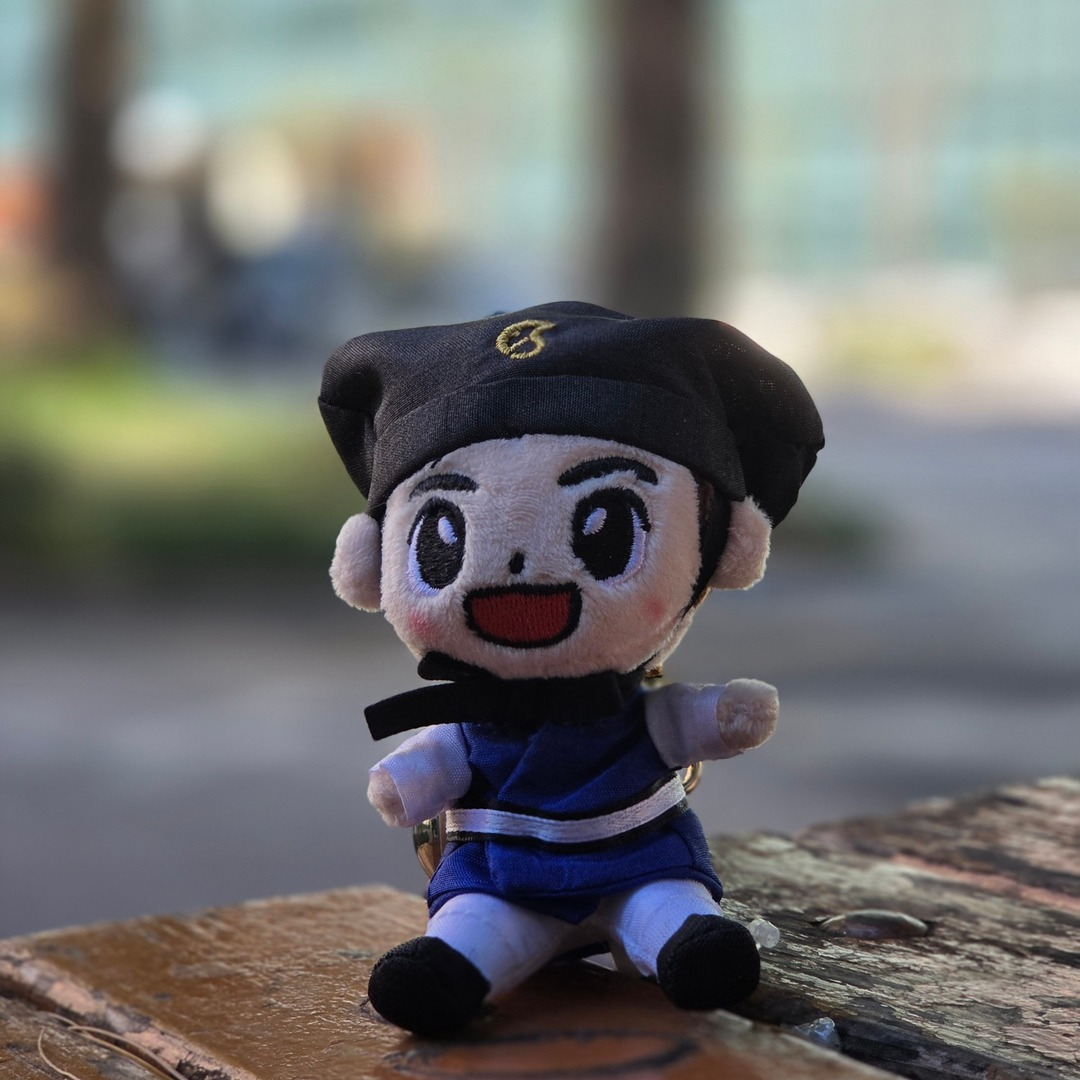
\includegraphics[width=0.325\columnwidth]{figures/fig_draft_final_gap_final.jpg}};
      \begin{scope}[x={(im.south east)}, y={(im.north west)}]
        \draw[orange, line width=0.8pt] (0.15,0.6435) rectangle (0.65,0.8102);
      \end{scope}
    \end{tikzpicture} &
    \begin{tikzpicture}
      \node[inner sep=0, anchor=south west] (im) at (0,0)
        {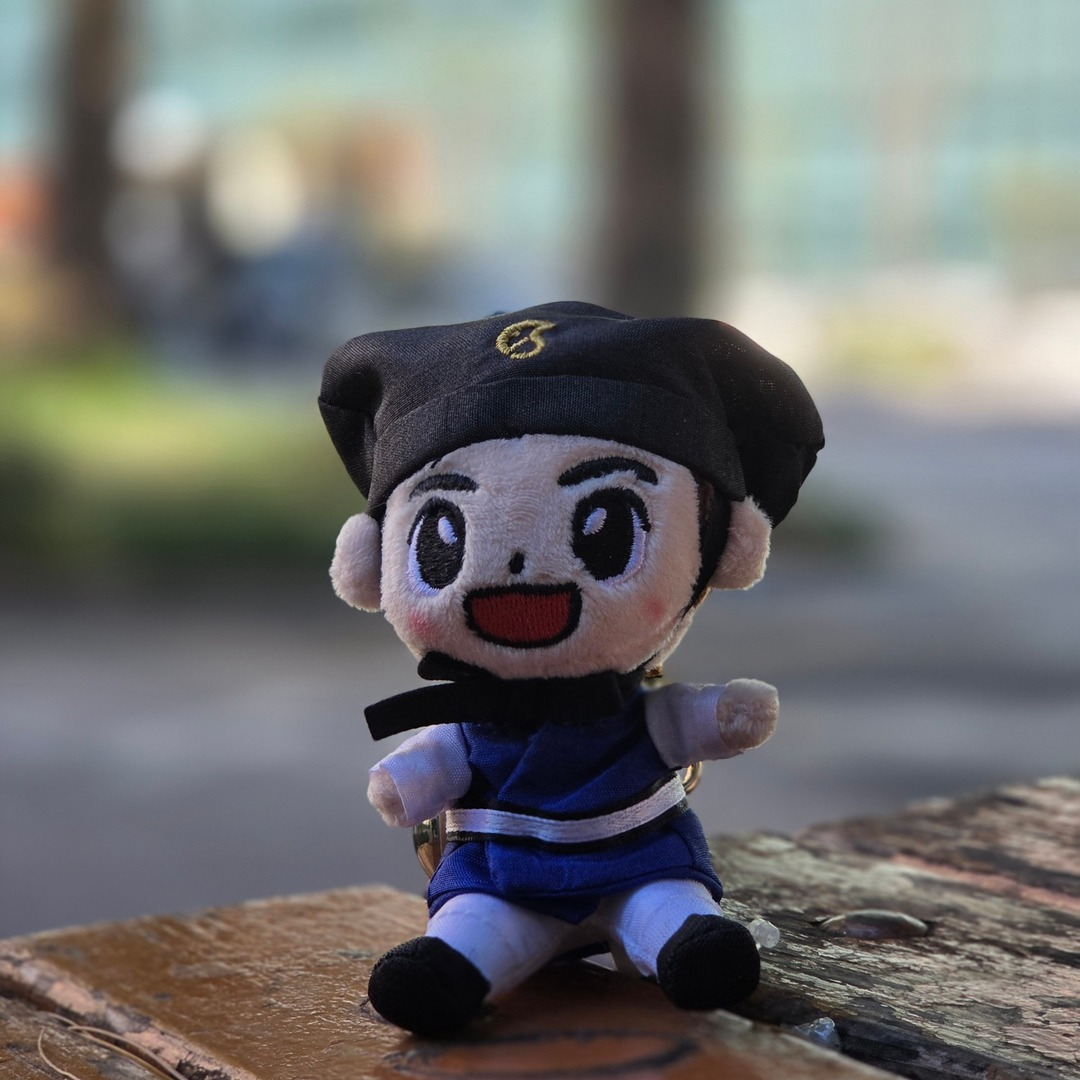
\includegraphics[width=0.325\columnwidth]{figures/fig_draft_final_gap_final.jpg}};
      \begin{scope}[x={(im.south east)}, y={(im.north west)}]
        \draw[orange, line width=0.8pt] (0.15,0.6435) rectangle (0.65,0.8102);
      \end{scope}
    \end{tikzpicture} \tabularnewline[1pt]
    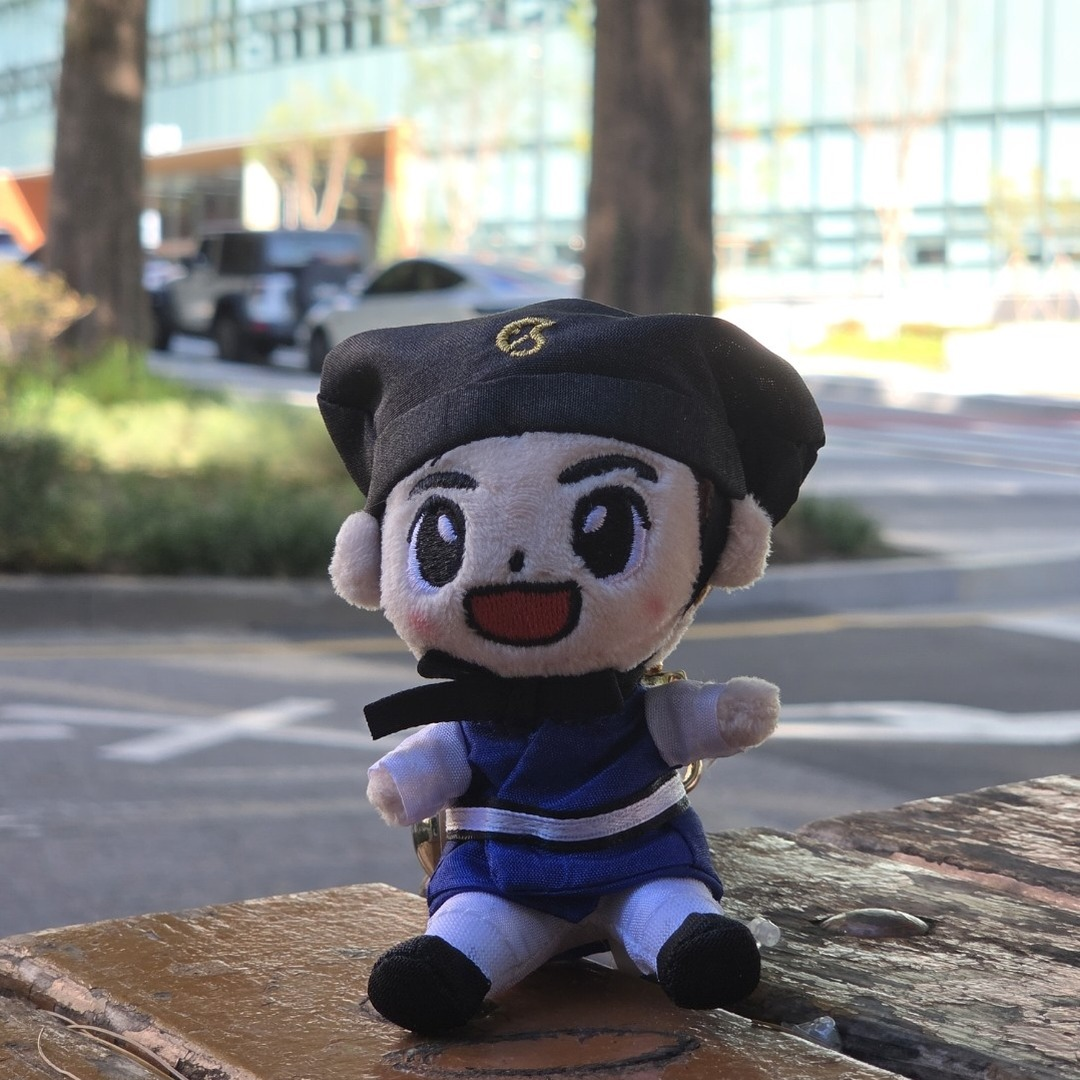
\includegraphics[width=0.325\columnwidth, trim=162 695 378 205, clip]{figures/fig_draft_final_gap_draft.jpg} &
    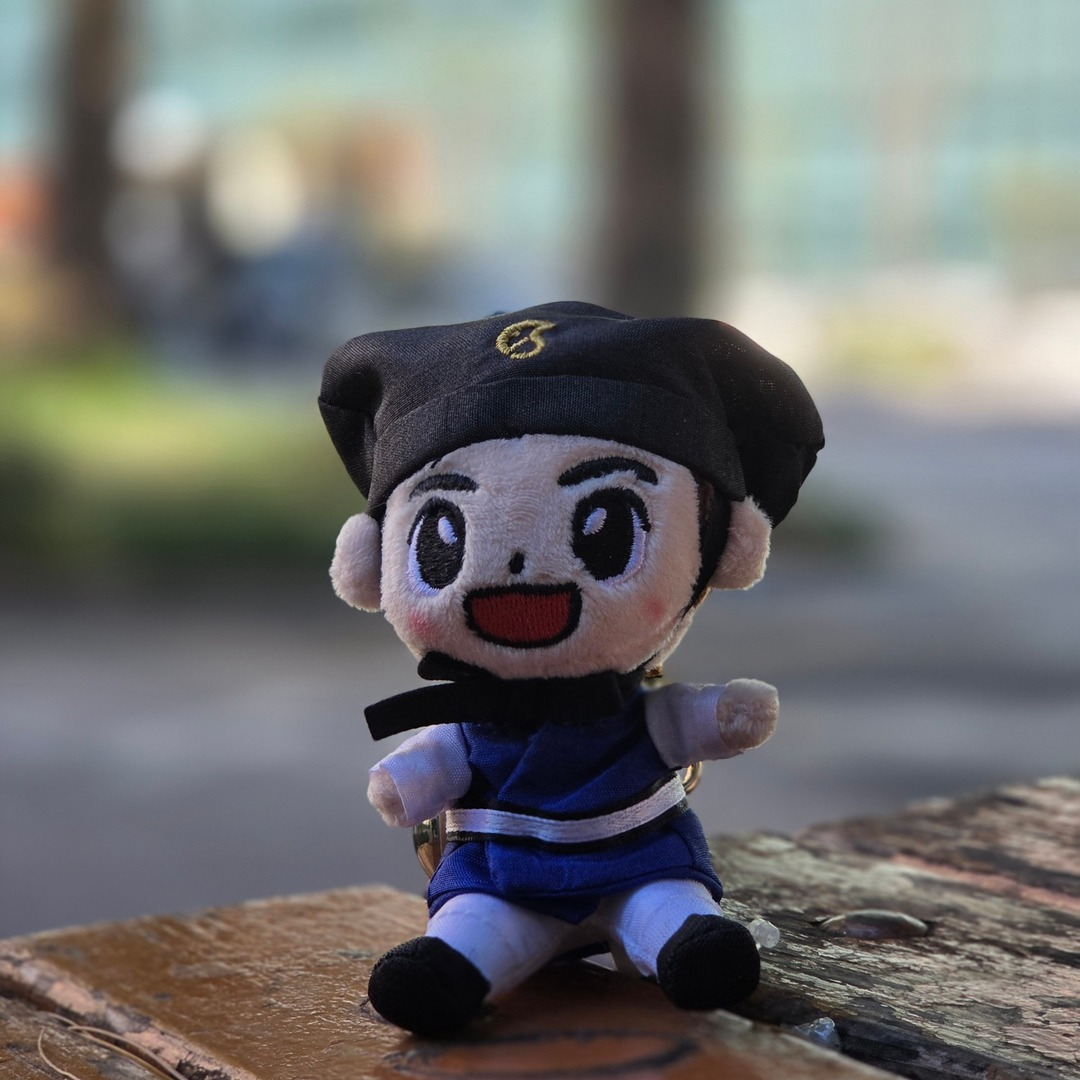
\includegraphics[width=0.325\columnwidth, trim=162 695 378 205, clip]{figures/fig_draft_final_gap_final.jpg} &
    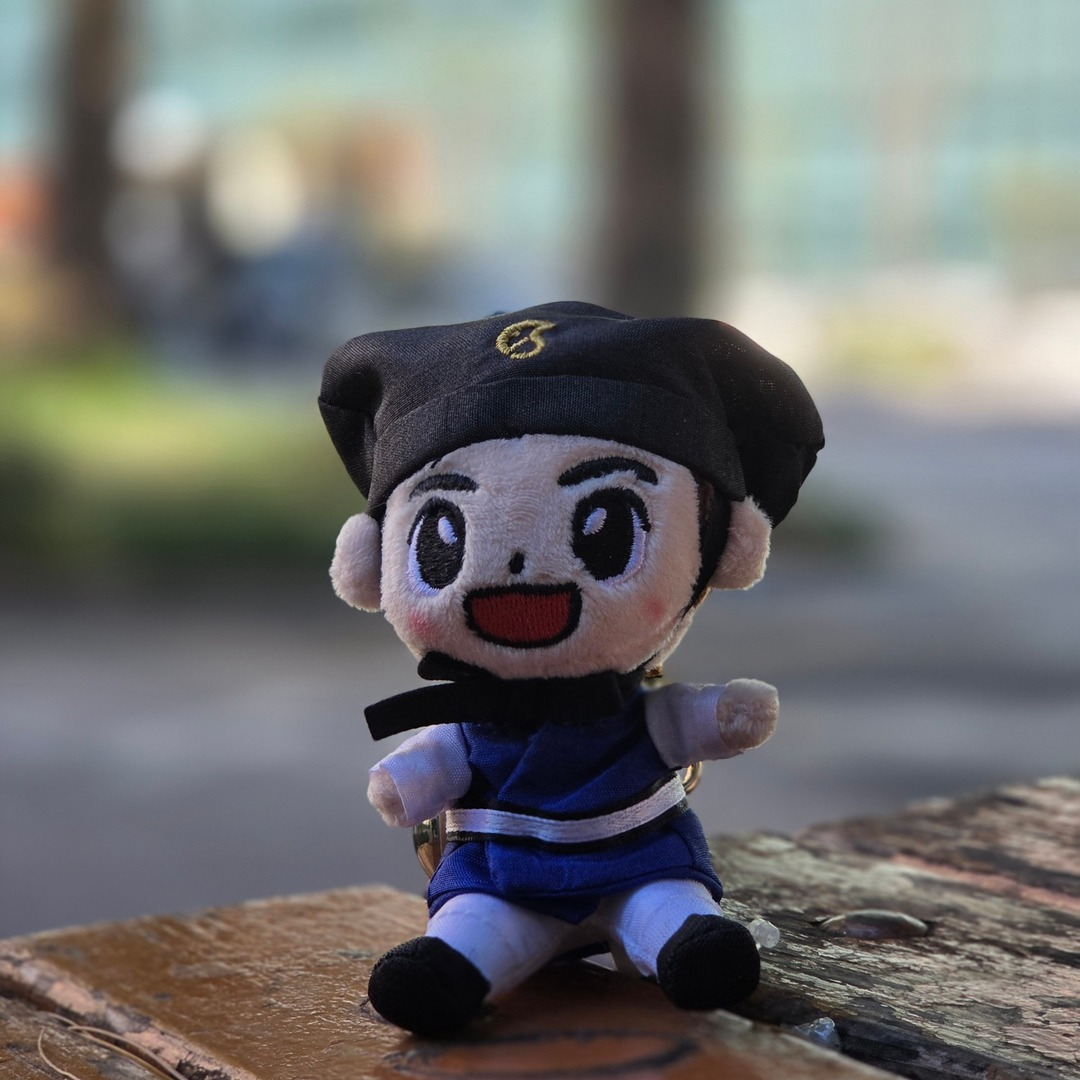
\includegraphics[width=0.325\columnwidth, trim=162 695 378 205, clip]{figures/fig_draft_final_gap_final.jpg}
    \tabularnewline[2pt]
    \parbox[t]{0.325\columnwidth}{\centering\scriptsize (a) Draft image} &
    \makebox[0.325\columnwidth][c]{%
      \parbox[t]{0.41\columnwidth}{\centering\scriptsize
        (b) Draft image with \\lightweight multi-frame composition}} &
    \parbox[t]{0.325\columnwidth}{\centering\scriptsize (c) Final image}
  \end{tabular}
  \caption{Draft--final visual differences in Portrait mode.}
  \label{fig:draft-final-gap}
\end{figure}


\smallskip\noindent\textbf{Extending the draft sequence.}
To reduce this gap, Samsung first added single-frame stages, such as Filter and Watermark, to the draft sequence.
Samsung then implemented lightweight multi-frame composition for Portrait mode to reduce the gap further (Figure~\ref{fig:draft-final-gap}(b)).
However, this additional processing can cause a Capture Timeout, particularly under parallel capture (Section~\ref{sec:parallel-capture}), so the feature has not been deployed on any device model.

% \subsection{Parallel Capture}
\label{sec:parallel-capture}

Parallel capture allows the camera application to accept the next shutter input before the preceding capture has produced its draft image.
This is possible because the hardware abstraction layer (HAL) can issue a capture-availability signal, \texttt{captureAvailable}, before the draft sequence completes.
This signal indicates when the application may accept the next capture request, allowing a shorter shot-to-shot interval.

However, draft sequences execute one at a time on a single draft worker to preserve capture order and limit peak memory demand.
When capture requests arrive faster than the worker completes draft sequences, later captures must wait in the draft queue.
Since each capture's timeout clock starts when its request is accepted, this wait consumes part of its timeout budget before its draft sequence starts.
Figure~\ref{fig:overlap} illustrates how this waiting time grows across successive captures even when their draft sequences take equally long.
Accumulated waiting time can therefore cause later captures to miss their deadlines, especially when lightweight multi-frame composition increases the draft processing time of earlier captures.

\begin{figure}[t]
  \centering
  \resizebox{\columnwidth}{!}{% Notes: docs/exhibits.md#fig_parallel_capture_overlap
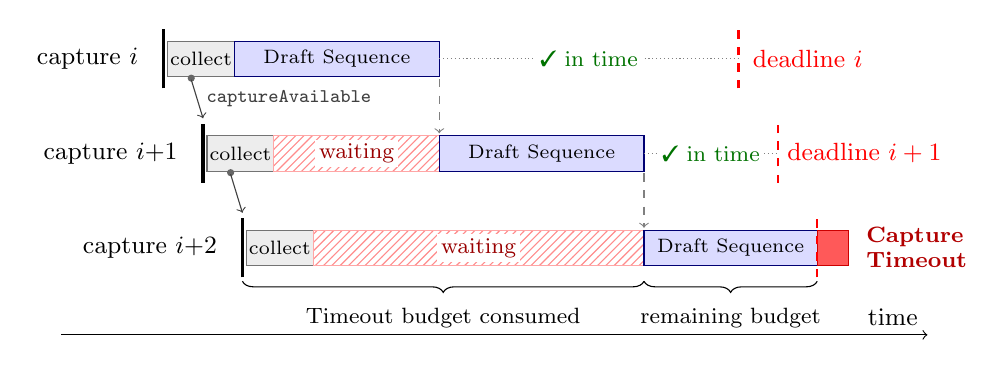
\begin{tikzpicture}[font=\small,
  collectstage/.style={draw=black!55, fill=gray!14},
  draftstage/.style={draw=blue!45!black, fill=blue!14},
  queued/.style={pattern=north east lines, pattern color=red!45, draw=red!35},
  overrun/.style={draw=red!80!black, fill=red!65},
  ddl/.style={red, dashed, thick},
  sig/.style={->, black!75}]

  \node[anchor=east] at (-0.2, 3.925) {capture $i$};
  \draw[very thick] (0, 3.55) -- (0, 4.30);
  \draw[collectstage] (0.05, 3.70) rectangle (0.90, 4.15);
  \node at (0.475, 3.925) {\scriptsize collect};
  \draw[draftstage] (0.90, 3.70) rectangle (3.50, 4.15);
  \node at (2.20, 3.925) {\scriptsize Draft Sequence};

  \draw[densely dotted, gray] (3.50, 3.925) -- (7.30, 3.925);
  \node[fill=white, inner sep=1.5pt] at (5.40, 3.925)
    {\footnotesize\textcolor{green!45!black}{\ding{51} in time}};
  \draw[ddl] (7.30, 3.55) -- (7.30, 4.30);
  \node[red, anchor=east] at (9.00, 3.925) {deadline $i$};

  \fill[black!60] (0.35, 3.68) circle (1.3pt);
  \draw[sig] (0.35, 3.66) -- (0.50, 3.17);
  \node[anchor=west, black!75] at (0.42, 3.42)
    {\scriptsize\texttt{captureAvailable}};

  \node[anchor=east] at (0.3, 2.725) {capture $i{+}1$};
  \draw[very thick] (0.50, 2.35) -- (0.50, 3.10);
  \draw[collectstage] (0.55, 2.50) rectangle (1.40, 2.95);
  \node at (0.975, 2.725) {\scriptsize collect};
  \draw[queued] (1.40, 2.50) rectangle (3.50, 2.95);
  \node[fill=white, inner sep=1.5pt] at (2.45, 2.725)
    {\footnotesize\textcolor{red!60!black}{waiting}};
  \draw[draftstage] (3.50, 2.50) rectangle (6.10, 2.95);
  \node at (4.80, 2.725) {\scriptsize Draft Sequence};

  \draw[densely dotted, gray] (6.10, 2.725) -- (7.80, 2.725);
  \node[fill=white, inner sep=1.5pt] at (6.95, 2.725)
    {\footnotesize\textcolor{green!45!black}{\ding{51} in time}};
  \draw[ddl] (7.80, 2.35) -- (7.80, 3.10);
  \node[red, anchor=east] at (10.00, 2.725) {deadline $i+1$};

  \fill[black!60] (0.85, 2.48) circle (1.3pt);
  \draw[sig] (0.85, 2.46) -- (1.00, 1.97);

  \node[anchor=east] at (0.8, 1.525) {capture $i{+}2$};
  \draw[very thick] (1.00, 1.15) -- (1.00, 1.90);
  \draw[collectstage] (1.05, 1.30) rectangle (1.90, 1.75);
  \node at (1.475, 1.525) {\scriptsize collect};
  \draw[queued] (1.90, 1.30) rectangle (6.10, 1.75);
  \node[fill=white, inner sep=1.5pt] at (4.00, 1.525)
    {\footnotesize\textcolor{red!60!black}{waiting}};
  \draw[draftstage] (6.10, 1.30) rectangle (8.70, 1.75);

  \draw[overrun] (8.30, 1.30) rectangle (8.70, 1.75);
  \node at (7.20, 1.525) {\scriptsize Draft Sequence};
  \draw[ddl] (8.30, 1.15) -- (8.30, 1.90);
  \node[red!70!black, anchor=west, align=left] at (8.80, 1.525)
    {\footnotesize\bfseries Capture\\[-2pt]\footnotesize\bfseries Timeout};

  \draw[dashed, gray, ->] (3.50, 3.67) -- (3.50, 2.98);
  \draw[dashed, gray, ->] (6.10, 2.47) -- (6.10, 1.78);

  \draw[decorate, decoration={brace, mirror, amplitude=4pt}]
    (1.00, 1.10) -- (6.10, 1.10);
  \node[anchor=north] at (3.55, 0.88) {\footnotesize Timeout budget consumed};
  \draw[decorate, decoration={brace, mirror, amplitude=4pt}]
    (6.10, 1.10) -- (8.30, 1.10);
  \node[anchor=north] at (7.20, 0.88) {\footnotesize remaining budget};

  \draw[->] (-1.3, 0.42) -- (9.7, 0.42) node[anchor=south east] {time};

\end{tikzpicture}
}
  \caption{Timeout budget consumed by queueing under parallel capture.}
  \label{fig:overlap}
\end{figure}

% \subsection{Limitations of the Thermal Guard}
\label{sec:guard-limit}

Samsung uses a static thermal guard to prevent Capture Timeout violations in deployed single-frame draft stages.
The guard uses Samsung's overheat level, an ordinal thermal indicator on a 0--6 scale, where larger values denote stronger throttling.
During pre-release validation, throttling at level~4 repeatedly delayed a single-frame draft stage and caused Capture Timeout violations despite optimization.
The guard therefore skips optional single-frame stages at level~4 or higher.

However, the overheat level does not indicate a capture's waiting time or remaining draft work.
The guard may therefore skip optional stages even when enough time remains to complete the draft sequence.
For example, ambient heat, charging, or prior heavy device workloads can readily raise the overheat level to 4 before a camera session starts.
The guard then skips optional stages on the session's first capture, even when its remaining timeout budget is sufficient.

\smallskip\noindent\textbf{Motivating experiment.}
To examine the timeout risk of enabling lightweight multi-frame composition in the draft sequence, we compared two Portrait configurations on the Galaxy S26 Ultra.
We bypassed the thermal guard so that configured optional stages could execute regardless of the overheat level.
The optional stages are the multi-frame composition stage (\(M\)) and the deployed single-frame stages (collectively \(S\)).
Both \(M\) alone and \(M+S\) retain the same mandatory encoding and saving stages.
We tested 12MP and 24MP capture under normal memory conditions and under memory pressure.
For each condition in Table~\ref{tab:timeout_index}, we ran ten trials of up to 30 consecutive captures.
We chose 30 captures to extend testing beyond the earlier level-4 validation failure near the 20th consecutive capture.
The table reports the earliest timeout capture index across the ten trials, grouped by starting overheat level.

% Notes: docs/exhibits.md#tab_timeout_index
\providecolor{tmoS1}{RGB}{252,227,220} %
\providecolor{tmoS2}{RGB}{239,160,140} %
\providecolor{tmoS3}{RGB}{201,80,63}  %
\providecolor{tmoS4}{RGB}{143,36,32}  %

\newcolumntype{H}{>{\centering\arraybackslash}m{1.20cm}}
\newcolumntype{P}{>{\centering\arraybackslash}m{0.67cm}}

\providecommand{\tmoFirst}[2]{\cellcolor{#1}\makebox[\linewidth][r]{#2\hspace{1pt}}}
\providecommand{\tmoFirstW}[2]{\cellcolor{#1}\makebox[\linewidth][r]{\textcolor{white}{\textbf{#2}}\hspace{1pt}}}
\providecommand{\tmoNone}{\makebox[\linewidth][r]{--\hspace{1pt}}}

\begin{table}[t]
 \centering
 \caption{Capture index of the earliest timeout.}
 \label{tab:timeout_index}
 {\scriptsize\setlength{\tabcolsep}{1.3pt}%
 \begin{tabular}{@{}HPP|PP||PP|PP@{}}
 \toprule
 \multirow[c]{3}{=}[-10pt]{\makecell[c]{\textbf{Starting}\\\textbf{overheat}\\\textbf{level}}} &
 \multicolumn{4}{c||}{\raisebox{-3pt}{\textbf{Normal capture}}} &
 \multicolumn{4}{c@{}}{\raisebox{-3pt}{\textbf{Memory-pressure capture}}} \\[6pt] \cmidrule(lr){2-5}\cmidrule(l){6-9}
 &
 \multicolumn{2}{c|}{\raisebox{-3pt}{\textbf{12MP}}} &
 \multicolumn{2}{c||}{\raisebox{-3pt}{\textbf{24MP}}} &
 \multicolumn{2}{c|}{\raisebox{-3pt}{\textbf{12MP}}} &
 \multicolumn{2}{c@{}}{\raisebox{-3pt}{\textbf{24MP}}} \\[6pt] \cmidrule(lr){2-3}\cmidrule(lr){4-5}\cmidrule(lr){6-7}\cmidrule(l){8-9}
 & \raisebox{-2pt}{\textbf{M{+}S}} & \raisebox{-2pt}{\textbf{M}} &
 \raisebox{-2pt}{\textbf{M{+}S}} & \raisebox{-2pt}{\textbf{M}} &
 \raisebox{-2pt}{\textbf{M{+}S}} & \raisebox{-2pt}{\textbf{M}} &
 \raisebox{-2pt}{\textbf{M{+}S}} & \raisebox{-2pt}{\textbf{M}} \\[4pt]
 \midrule
 Lv0 &
 \tmoNone & \tmoNone & \tmoFirst{tmoS1}{29} & \tmoNone &
 \tmoNone & \tmoNone & \tmoFirst{tmoS1}{26} & \tmoNone \\
 Lv1 &
 \tmoNone & \tmoNone & \tmoFirst{tmoS1}{29} & \tmoNone &
 \tmoFirst{tmoS1}{24} & \tmoNone & \tmoFirst{tmoS2}{19} & \tmoNone \\
 Lv2 &
 \tmoFirst{tmoS1}{24} & \tmoNone & \tmoFirst{tmoS2}{18} & \tmoNone &
 \tmoFirst{tmoS2}{15} & \tmoFirst{tmoS1}{29} &
 \tmoFirst{tmoS2}{14} & \tmoFirst{tmoS1}{25} \\
 Lv3 &
 \tmoFirst{tmoS2}{13} & \tmoFirst{tmoS1}{21} &
 \tmoFirst{tmoS2}{12} & \tmoFirst{tmoS1}{20} &
 \tmoFirstW{tmoS3}{8} & \tmoFirst{tmoS2}{19} &
 \tmoFirstW{tmoS4}{5} & \tmoFirst{tmoS2}{13} \\
 \midrule
 Lv4 &
 \tmoFirstW{tmoS3}{8} & \tmoFirst{tmoS2}{16} &
 \tmoFirstW{tmoS3}{7} & \tmoFirst{tmoS2}{13} &
 \tmoFirstW{tmoS3}{6} & \tmoFirst{tmoS2}{13} &
 \tmoFirstW{tmoS4}{3} & \tmoFirstW{tmoS3}{7} \\
 Lv5 &
 \tmoFirstW{tmoS3}{8} & \tmoFirst{tmoS2}{12} &
 \tmoFirstW{tmoS3}{8} & \tmoFirst{tmoS2}{12} &
 \tmoFirstW{tmoS4}{4} & \tmoFirstW{tmoS3}{9} &
 \tmoFirstW{tmoS4}{4} & \tmoFirstW{tmoS3}{9} \\
 Lv6 &
 \tmoFirstW{tmoS3}{7} & \tmoFirst{tmoS2}{11} &
 \tmoFirstW{tmoS3}{7} & \tmoFirst{tmoS2}{11} &
 \tmoFirstW{tmoS4}{3} & \tmoFirstW{tmoS3}{6} &
 \tmoFirstW{tmoS4}{3} & \tmoFirstW{tmoS3}{6} \\
 \bottomrule
 \end{tabular}%
 }
 \par\vspace{3pt}
 {\scriptsize\begin{minipage}{0.933\columnwidth}
 \raggedright\setlength{\fboxsep}{1.8pt}%
 Timeout capture index:~%
 \colorbox{tmoS1}{\strut\,${\geq}\,20$\,}\colorbox{tmoS2}{\strut\,10--19\,}\colorbox{tmoS3}{\strut\,\textcolor{white}{6--9}\,}\colorbox{tmoS4}{\strut\,\textcolor{white}{${\leq}\,5$}\,}\par
 --: no timeout observed within 30 captures.\par
 \end{minipage}}
\end{table}


The overheat level alone was insufficient to explain timeout onset.
With \(M+S\), timeouts occurred even in runs starting below the guard's cutoff.
Conversely, every \(M+S\) trial starting at level~4 or higher completed its first capture without a timeout.
At the same starting level on the same device, the earliest timeout varied with resolution, memory pressure, and draft configuration.
In particular, compared with \(M+S\), using \(M\) alone delayed the earliest timeout or resulted in no observed timeout within 30 captures.

\smallskip\noindent\textbf{Need for runtime control.}
The experiment shows that reducing optional draft work can delay timeout onset.
However, skipping optional stages can widen the draft--final visual gap and cannot recover timeout budget already spent waiting.
Delaying the next capture opportunity can limit draft queue growth and preserve budget for optional processing, at the cost of a longer shot-to-shot interval.
These trade-offs motivate coordinated runtime control of optional-stage execution and capture arrivals.
To determine how much timeout budget to reserve, both decisions require estimating the time needed for the remaining draft work.
Reserving too little risks a Capture Timeout, whereas reserving too much needlessly sacrifices draft image quality or capture responsiveness.


\section{The Budget-Aware Draft Controller}
\label{sec:approach}

\subsection{Overview}
\label{sec:objective}

\begin{figure*}[!t]
  \centering
  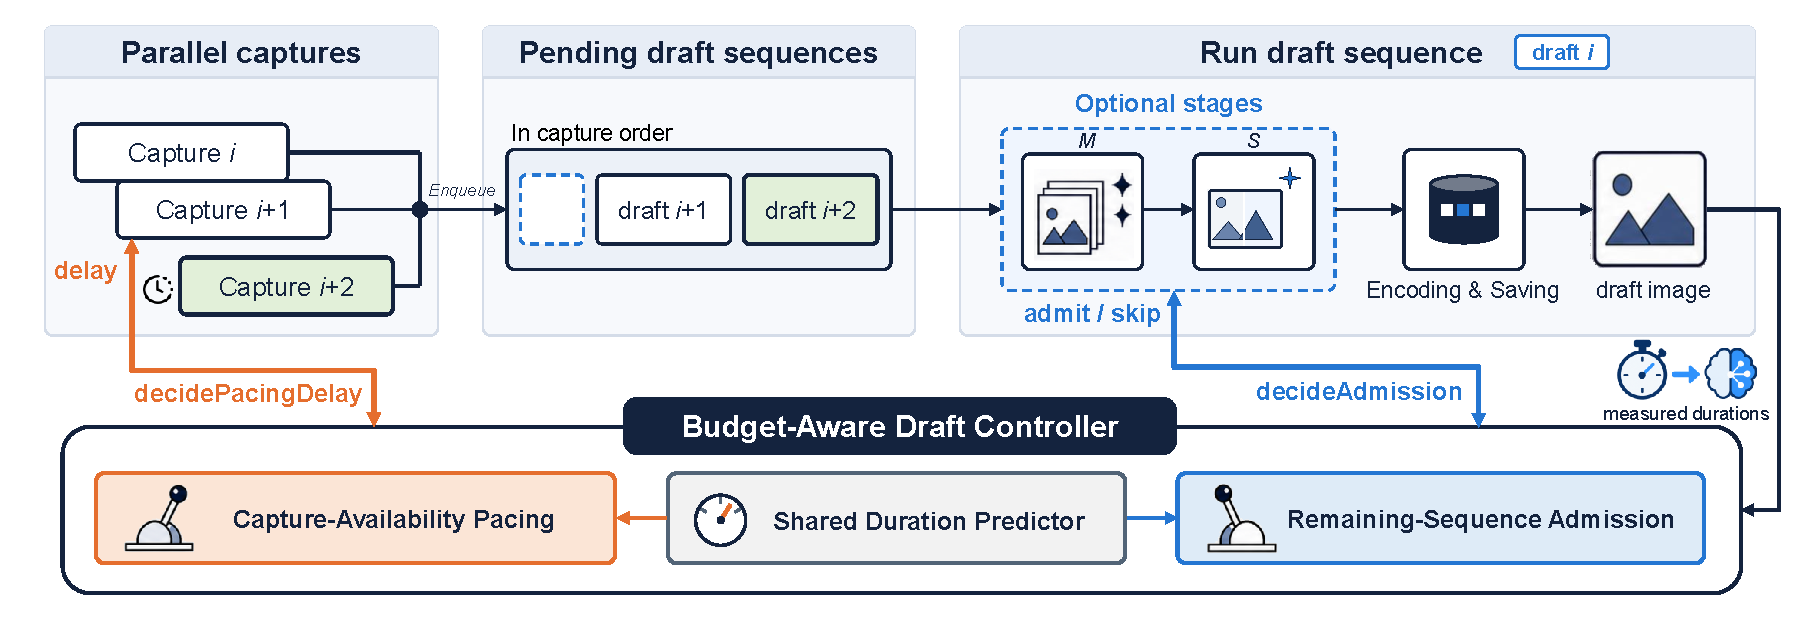
\includegraphics[trim=12 10 0 11,clip,width=\textwidth]{figures/fig_controller_interaction.pdf}
  \caption{Coordinated Admission and Pacing in the Budget-Aware Draft Controller.}
  \label{fig:controller-overview}
\end{figure*}
Figure~\ref{fig:controller-overview} illustrates how the \emph{Budget-Aware Draft Controller} coordinates optional-stage execution with capture arrivals.
The controller combines \emph{Remaining-Sequence Admission}, which decides whether optional stages execute, with \emph{Capture-Availability Pacing}, which regulates the next capture opportunity.
Both use a shared duration predictor updated from measured durations in the current camera session, without per-device timing tables.
The controller is integrated at two existing points: before optional-stage execution and before \texttt{captureAvailable} delivery.
This integration preserves the draft pipeline structure and the existing HAL and application interfaces.

Algorithm~\ref{alg:overview} locates the controller's decisions and state updates within the capture workflow.
At acceptance of request \(i\), the workflow sets \(\mathit{timeout}_i=\mathit{now}+\textsc{TIMEOUT}\), where \textsc{TIMEOUT} is the fixed Capture Timeout duration (line~\ref{alg:ov:timeout}).
When \texttt{captureAvailable} is ready for delivery, \(\mathit{controller}.\textsc{DecidePacingDelay}\) computes \(\mathit{delay}_i\) from projected draft workload and the remaining timeout budget of the capture whose draft sequence was most recently enqueued in the draft queue (line~\ref{alg:ov:pacing}).
\textsf{ScheduleCaptureAvailable} schedules the callback for delivery after this delay, exposing the next capture opportunity \(i+1\) to the application (line~\ref{alg:ov:notify}).
The original workflow delivers the callback immediately (\(\mathit{delay}_i=0\)).

Algorithm~\ref{alg:overview} presents the control flow of each capture in logical order.
It does not imply that captures are processed sequentially.
Although draft execution and its completion update appear inline (lines~\ref{alg:ov:configure}--\ref{alg:ov:update}), sequences are enqueued for the single draft worker and executed in capture order (Section~\ref{sec:parallel-capture}).
Draft processing therefore proceeds without waiting for \(\mathit{delay}_i\), and later captures can arrive before capture \(i\)'s draft sequence completes.

\input{figures/alg_overview.tex}

At sequence start, \textsf{ConfigureDraftStages} obtains the configured sequence \(\mathcal K_i=(k_1,\ldots,k_m)\) (line~\ref{alg:ov:configure}), whose keys identify stages and their configurations.
The original workflow excludes optional stages from \(\mathcal K_i\) at overheat level~4 or higher.
The controller instead keeps configured optional stages in \(\mathcal K_i\) and decides their execution through runtime admission.
Before each optional stage \(k_j\), \(\mathit{controller}.\textsc{DecideAdmission}\) compares the estimated duration of the remaining sequence \(\mathcal K_{i,j}=(k_j,\ldots,k_m)\) with the remaining timeout budget \(T_{i,j}\) (line~\ref{alg:ov:admission}).
\textsf{CompleteDraftSequence} performs the mandatory encoding and saving, represented by the final key \(k_m\), to produce the draft image \(\mathit{draft}_i\) (line~\ref{alg:ov:publish}).

Along with \(\mathit{draft}_i\), \textsf{CompleteDraftSequence} returns the measured durations \(p_i(k)\) of the executed stages in \(\mathcal K_i\) and the draft sequence duration \(C_i\).
At line~\ref{alg:ov:update}, \(\mathit{controller}.\textsc{Update}\) uses these measurements to update the shared predictor and the admission and pacing states for subsequent decisions.

\smallskip\noindent\textbf{Control objective.}
The control objective is to complete each capture's draft sequence before its Capture Timeout deadline and, within that constraint, to weigh capture responsiveness more heavily than optional-stage retention.
Deadline safety comes first because a single Capture Timeout violation blocks the release.
Responsiveness has higher priority because added shot-to-shot delay is irreversible, whereas skipping optional stages lowers draft quality but leaves the final image unaffected.
Let \(\mu_i\) be the time left before capture \(i\)'s deadline at draft completion, \(\delta_i\) the interval between acceptance of requests \(i-1\) and \(i\), and \(\pi_i\) the interval between their draft completions.
With a fixed timeout duration,
\begin{equation}
  \mu_i=\mu_{i-1}+\delta_i-\pi_i .
  \label{eq:margin-recursion}
\end{equation}
When \(\pi_i>\delta_i\), the deadline margin shrinks.
Repeated decreases can exhaust the deadline margin and cause a Capture Timeout.
Admission can shorten \(\pi_i\) by skipping optional stages but cannot recover time already spent waiting.
Pacing can lengthen \(\delta_{i+1}\) by delaying the next capture opportunity but cannot change work in progress.
Admitted optional work affects workload estimates for later pacing delays, so the controller coordinates admission and pacing to avoid exhausting the margin.

\subsection{Shared Duration Predictor}
\label{sec:model}
The controller's \emph{shared duration predictor} provides stage-duration estimates for both admission and pacing.
Because draft processing time varies with stage configuration and runtime conditions (Section~\ref{sec:guard-limit}), the predictor updates these estimates online from completed draft sequences.
Admission applies them to the remaining sequence \(\mathcal K_{i,j}\), while pacing uses them to predict queued and upcoming draft work.
Algorithm~\ref{alg:shared-predictor} shows how the predictor computes and updates these estimates.

\begin{algorithm}[t]
\caption{Shared Duration Predictor}
\label{alg:shared-predictor}
\footnotesize
\renewcommand{\algorithmicrequire}{\textbf{Input:}}
\renewcommand{\algorithmicensure}{\textbf{Output:}}
\algtext*{EndFunction}\algtext*{EndProcedure}\algtext*{EndIf}\algtext*{EndFor}
\begin{algorithmic}[1]
\Require Workload sequence ($\mathcal K$), measured stage durations ($p_i$)
\Ensure Point estimate ($\hat P$)
\State $\hat b(k)\gets0\ (\forall k),\quad \gamma\gets1$ \label{alg:pe:init}
\State
\Function{ComputePointEstimate}{$\mathcal K$}
  \State \Return $\sum_{k\in\mathcal K}\hat b(k)\cdot\gamma$ \label{alg:pe:compute}
\EndFunction
\State
\Procedure{Update}{$\mathcal K_i,p_i$}
  \State $\gamma_{\mathrm{old}}\gets\gamma,\quad \mathit{ratios}\gets\emptyset$ \label{alg:pe:snapshot}
  \For{each workload key $k\in\mathcal K_i$ with $p_i(k)>0$} \label{alg:pe:loop}
    \If{$\hat b(k)>0$} \label{alg:pe:observed}
      \State $\mathit{ratios}\gets\mathit{ratios}\uplus\{p_i(k)/\hat b(k)\}$ \label{alg:pe:ratio}
    \EndIf
    \State $\hat b(k)\gets$ cumulative average including $p_i(k)/\gamma_{\mathrm{old}}$ \label{alg:pe:base}
  \EndFor
  \If{$\mathit{ratios}\neq\emptyset$} \label{alg:pe:condition}
    \State $\gamma\gets\operatorname{median}(\mathit{ratios})$ \label{alg:pe:gamma}
  \EndIf
\EndProcedure
\end{algorithmic}
\end{algorithm}


\smallskip\noindent\textbf{Point estimate.}
The predictor models each stage duration as a key-specific base duration \(\hat b(k)\) scaled by a factor \(\gamma\) shared across keys.
The base duration captures timing differences among stages and configurations, while \(\gamma\) provides a shared adjustment for changes in runtime conditions.
At line~\ref{alg:pe:init}, Algorithm~\ref{alg:shared-predictor} initializes every base duration to zero and \(\gamma\) to one.
For a workload sequence \(\mathcal K\), \textsc{ComputePointEstimate} (line~\ref{alg:pe:compute}) returns the point estimate \(\hat P(\mathcal K)\), the sum of the predicted stage durations \(\hat p(k)\):
\begin{equation*}
  \hat P(\mathcal{K})
  =\sum_{k\in\mathcal{K}}\hat p(k),
  \qquad
  \hat p(k)=\hat b(k)\,\gamma .
\end{equation*}

\smallskip\noindent\textbf{Online predictor update.}
The base duration \(\hat b(k)\) accumulates normalized measurements of its key, whereas \(\gamma\) reflects the latest available measurement-to-base ratios.
At draft completion, \(\mathit{controller}.\textsc{Update}\) first updates the predictor using measured stage durations \(p_i(k)\) (Algorithm~\ref{alg:overview}, line~\ref{alg:ov:update}).
For each key with \(p_i(k)>0\), the predictor collects \(p_i(k)/\hat b(k)\) in \(\mathit{ratios}\) if \({\hat b(k)>0}\), before updating the base duration (Algorithm~\ref{alg:shared-predictor}, line~\ref{alg:pe:ratio}).
It then incorporates \(p_i(k)/\gamma_{\mathrm{old}}\), where \(\gamma_{\mathrm{old}}\) is \(\gamma\) before this update, into the cumulative average \(\hat b(k)\) (Algorithm~\ref{alg:shared-predictor}, line~\ref{alg:pe:base}).
Finally, if \(\mathit{ratios}\) is nonempty, the predictor replaces \(\gamma\) with the median of \(\mathit{ratios}\) (Algorithm~\ref{alg:shared-predictor}, line~\ref{alg:pe:gamma}).
The cumulative average \(\hat b(k)\) dampens isolated spikes in a key's duration history, and when multiple ratios are available, their median \(\gamma\) limits the influence of a single-stage deviation.

\subsection{Remaining-Sequence Admission}
\label{sec:admission}

Immediately before each optional stage, \emph{Admission} compares the capture's remaining timeout budget with the estimated duration of the entire remaining draft sequence, including mandatory encoding and saving.
This timing accounts for the budget consumed by queueing and earlier stages.

\smallskip\noindent\textbf{Admission rule.}
The point estimate \(\hat P(\mathcal K_{i,j})\) may underestimate the time needed to finish the remaining sequence.
Admission therefore uses an empirical upper estimate \(U(\mathcal K_{i,j})\) of the remaining processing time for the budget comparison.
\(\mathit{controller}.\textsc{DecideAdmission}\) (Algorithm~\ref{alg:overview}, line~\ref{alg:ov:admission}) admits an optional stage \(k_j\) when
\begin{equation}
  U(\mathcal{K}_{i,j})\leq T_{i,j}
  \quad\text{or}\quad
  \hat P(\mathcal{K}_{i,j})=0.
  \label{eq:admission}
\end{equation}
When \(\hat P(\mathcal K_{i,j})=0\), the predictor has no prior timing measurements for the remaining enabled stages, so the optional stage is admitted to collect initial measurements.
This rule assumes that each configuration can complete an isolated first capture within the Capture Timeout, a capture-level requirement enforced by release validation (Section~\ref{sec:release-process}).

Admission treats \(M\) and \(S\) as separate groups.
Once an \(M\) or \(S\) stage is rejected, admission disables the optional stages in that group.
Until the draft queue drains, admission skips those stages and excludes them from subsequent \(\hat P\) and \(U\) estimates.
This avoids repeatedly toggling the group's visual effects across consecutive draft images.
When the queue drains, both groups are enabled again.

\smallskip\noindent\textbf{Upper-estimate calibration.}
Admission computes the upper estimate by multiplying the point estimate \(\hat P(\mathcal K)\) by an empirical residual factor \(\phi_\tau(\mathcal K)\geq1\):
\begin{equation}
  U(\mathcal{K})
  =\hat P(\mathcal{K})\,\phi_{\tau}(\mathcal{K}).
  \label{eq:upper-estimate}
\end{equation}
After the shared predictor is updated at draft completion, admission calibrates \(\phi_\tau\) for later decisions from observed stage overruns (Algorithm~\ref{alg:overview}, line~\ref{alg:ov:update}).
For each remaining sequence \(\mathcal K_{i,j}\), it forms a measured subsequence \(\mathcal K\) containing only executed stages (\(p_i(k)>0\)).
If \(\mathcal K\) contains a previously measured stage, admission computes a residual factor using the stage-duration predictions \(\hat p_i(k)\) retained before execution:
\begin{equation}
  \phi(\mathcal{K})
  =\frac{\sum_{k\in\mathcal{K}}\max\{\hat p_i(k),p_i(k)\}}
         {\sum_{k\in\mathcal{K}}\hat p_i(k)}.
  \label{eq:residual-factor}
\end{equation}
The per-key maximum preserves each stage's overrun even when another stage finishes faster than predicted, ensuring \(\phi(\mathcal{K})\geq1\).
Normalizing by the total predicted duration expresses stage overruns as a relative correction, making factors comparable across sequences with different predicted durations.

Admission maintains a residual-factor history for each measured sequence.
When a completion yields factors, admission multiplies all existing history weights by \(0.90\) to emphasize recent overruns.
We selected this decay factor at the knee of the trade-off between the overrun rate and the magnitude of \(U\).
Admission then inserts one factor per distinct measured sequence into its history with unit weight.
It selects each history's weighted \(\tau\)-quantile as its residual factor \(\phi_\tau\).
It determines \(\tau\) from the Kish effective sample size \(n_{\mathrm{eff}}\) of the current weights \(w_l\) in that history~\cite{kish-survey-sampling}:
\[
  n_{\mathrm{eff}}
  =\frac{(\sum_l w_l)^2}{\sum_l w_l^2},
  \qquad
  \tau=\frac{n_{\mathrm{eff}}}{n_{\mathrm{eff}}+1}.
\]
This choice of \(\tau\) is motivated by the expected CDF position \(n/(n+1)\) of the maximum of \(n\) i.i.d. continuous samples~\cite{david-order-statistics}, with \(n_{\mathrm{eff}}\) substituting for the sample count.
As the effective sample size grows, the selected quantile moves further into the observed upper tail.
Setting \(\tau\) this way avoids a separately tuned target percentile.
For a sequence without residual history, admission applies the same rule to residual factors pooled across sequences.
If no residual factors have been observed, it sets \(\phi_\tau(\mathcal K)=1\).

\smallskip\noindent\textbf{Watchdog fallback.}
An admitted stage may still run longer than predicted, and it cannot be cancelled once it enters native image processing.
The watchdog therefore triggers fallback if the stage has not completed within the following time budget:
\begin{equation}
  W_{i,j}=\max\{0,T_{i,j}-U(\mathcal{K}_{i,m})\},
  \label{eq:watchdog}
\end{equation}
where \(\mathcal{K}_{i,m}=(k_m)\), so \(U(\mathcal K_{i,m})\) reserves time for mandatory encoding and saving.
Fallback encodes and saves the preserved original input on a separate thread while the admitted stage continues running.
The resources held by the stage are released after it returns.
Queued draft sequences also bypass optional processing until the queue drains, reducing the risk that an overrun propagates to subsequent captures.

\subsection{Capture-Availability Pacing}
\label{sec:pacing}

\emph{Pacing} maintains a running forecast of draft workload to regulate the next capture opportunity.
It extends this forecast after each decision and rebases it as draft sequences complete.

\smallskip\noindent\textbf{Delay rule.}
When the \texttt{captureAvailable} callback for capture \(i\) is ready for delivery, \(\mathit{controller}.\textsc{DecidePacingDelay}\) (Algorithm~\ref{alg:overview}, line~\ref{alg:ov:pacing}) determines the callback delivery delay.
Pacing returns zero delay if the draft queue is empty or no draft sequence has completed.
Otherwise, it applies
\begin{equation*}
  \mathit{delay}_i
  =
  \left\lceil
    \frac{
      \max\{0,\hat B_i+2\hat R-T_{\mathrm{queue}}\}
    }{2}
  \right\rceil.
\end{equation*}

First, the predicted backlog \(\hat B_i\) estimates the time needed to drain draft work from earlier captures.
At each pacing decision, pacing computes this backlog as
\begin{equation*}
  \hat B_i
  =
  \max\{0,\hat t_{\mathrm{drain}}-\mathit{now}\},
\end{equation*}
where \(\hat t_{\mathrm{drain}}\) is the predicted drain time, computed from point estimates of draft work and updated by Equations~\eqref{eq:clock-update} and~\eqref{eq:clock-rebase}.

Second, pacing uses a conservative duration reserve \(\hat R\) per capture to project the draft workload added by the current capture \(i\) and the next capture \(i+1\) enabled by this callback.
Because \(\hat B_i\) does not yet include draft work for either capture, pacing adds \(\hat R\) for each, giving the projected workload \(\hat B_i+2\hat R\).
Pacing computes the reserve as
\begin{equation*}
  \hat R
  =
  \hat P(\mathcal K^{\mathrm{adm}})
  +
  \max\!\left(0,C_\tau-\hat P(\mathcal K)\right),
\end{equation*}
where \(\mathcal K^{\mathrm{adm}}\) is the subsequence of the configured sequence \(\mathcal K\) excluding optional work disabled by admission, and \(C_\tau\) is the recency-weighted \(\tau\)-quantile of completed draft-sequence durations.
Pacing applies the same recency weighting and selects \(\tau\) using the same effective-sample-size-based rule as admission does for residual factors in Section~\ref{sec:admission}.
The second term \(\max(0,C_\tau-\hat P(\mathcal K))\) adds empirical headroom because the draft sequences of captures \(i\) and \(i+1\) execute after the existing backlog and may encounter further thermal throttling.
With all configured stages enabled (\(\mathcal K^{\mathrm{adm}}=\mathcal K\)), pacing uses the larger of \(C_\tau\) and \(\hat P(\mathcal K)\) as its reserve.
After admission disables optional work, pacing adds the positive excess of \(C_\tau\) over \(\hat P(\mathcal K)\) as headroom to the point estimate \(\hat P(\mathcal K^{\mathrm{adm}})\).

Third, \(T_{\mathrm{queue}}\) denotes the remaining timeout budget of the most recently enqueued capture in the draft queue.
At the pacing decision point, capture \(i+1\)'s timeout clock has not yet started.
\(T_{\mathrm{queue}}\) therefore serves as a queue-level pressure reference for the projected workload \(\hat B_i+2\hat R\).
Pacing uses this pressure to limit queue growth, aiming to preserve time for capture \(i+1\)'s draft processing after acceptance.

Finally, pacing sets the callback delivery delay to half of the projected workload excess over the queue-level budget.
This heuristic aims to limit irreversible shot-to-shot latency, leaving workload reduction to admission.

\smallskip\noindent\textbf{Backlog extension.}
In the parallel capture workflow, the pacing decision for capture \(i+1\) may occur before capture \(i\)'s draft sequence is enqueued.
Pacing therefore provisionally extends \(\hat t_{\mathrm{drain}}\) after computing \(\mathit{delay}_i\) to include this work in subsequent delay calculations.
It uses \(\hat P^{\mathrm{last}}\), the value of \(\hat P(\mathcal K^{\mathrm{adm}})\) evaluated at the most recent draft completion:
\begin{equation}
  \hat t_{\mathrm{drain}}
  \gets
  \max\{\hat t_{\mathrm{drain}},\mathit{now}+\mathit{delay}_i\}
  +\lceil\hat P^{\mathrm{last}}\rceil.
  \label{eq:clock-update}
\end{equation}
The \(\max\) term anchors this provisional forecast to the later of the existing drain forecast \(\hat t_{\mathrm{drain}}\) and the callback delivery time \(\mathit{now}+\mathit{delay}_i\).
This keeps at least one draft sequence's predicted processing time in the provisional backlog when the next capture opportunity opens.
In this way, this extension accounts for the possibility that capture \(i\)'s draft sequence has not started by the callback delivery time.

\smallskip\noindent\textbf{Backlog rebase.}
Pacing rebases the backlog at each draft completion because provisional backlog extensions use earlier point estimates that can become stale as durations and admission state change.
After the shared predictor and admission update their states (Algorithm~\ref{alg:overview}, line~\ref{alg:ov:update}), pacing re-anchors the drain forecast at \(\mathit{now}\):
\begin{equation}
  \hat t_{\mathrm{drain}}
  \gets
  \mathit{now}
  +\left\lceil
    N_{\mathrm{pend}}\cdot\hat P(\mathcal K^{\mathrm{adm}})
  \right\rceil.
  \label{eq:clock-rebase}
\end{equation}
Here, \(N_{\mathrm{pend}}\) is the number of captures whose pacing decisions have occurred but whose draft sequences have not yet started.
Pacing increments this count after each pacing decision and decrements it when the corresponding draft sequence starts.
All pending captures share the configured sequence \(\mathcal K\), which cannot change until the draft queue drains.
Backlog rebase therefore refreshes the forecast for all pending captures using the latest duration estimates and admission state.


\input{_4_experiments}
\section{Related Work}
\label{sec:related_work}

\smallskip\noindent\textbf{Workload control.}
Workload control adapts the amount of computation under latency, resource, or thermal constraints~\cite{zilberstein-anytime,loop-perforation-fse,apnet-rtss,branchynet-icpr,approxdet-sensys,phoenix-tecs}, including reductions in per-request work under overload~\cite{abdelzaher-content-adaptation,klein-brownout}.
Imprecise computation separates mandatory and optional work, executing optional work when time permits~\cite{liu-imprecise-computation,shih-imprecise-siam}.
Timecard helps servers determine a request's processing budget from elapsed time and predicted downstream delay, leaving the adaptation mechanism service-specific~\cite{timecard-sosp}.
Before each non-preemptible optional draft stage, our admission checks whether the remaining timeout budget covers an empirical upper duration estimate for the entire remaining sequence, including mandatory encoding and saving.

\smallskip\noindent\textbf{Arrival control.}
Arrival control limits queue growth by regulating request release or admission.
Network senders pace packets to limit bursts and queue buildup~\cite{tcp-pacing-infocom,bbr-queue}, while servers throttle arrivals or shed requests under overload~\cite{seda-sosp,dagor-socc,breakwater-osdi}.
Real-time schedulers stretch task periods or skip jobs~\cite{buttazzo-elastic-task,koren-skip-over}.
Preemptive scheduling can also reduce queueing delay by interrupting long-running requests~\cite{shinjuku-nsdi}.
Our pacing regulates the next capture opportunity because accepted captures cannot be rejected and running stages cannot be preempted.

\smallskip\noindent\textbf{Coordinating workload and arrivals.}
Prior systems combine workload and arrival control.
Feedback-control schedulers adjust request admission and service levels using deadline-miss or utilization feedback~\cite{lu-feedback-control-edf,lu-feedback-control-scheduling}.
Server overload control adjusts admission and service quality against percentile response-time targets and can reject requests~\cite{welsh-overload-control}.
QoS negotiation selects among client-acceptable service levels and uses resource reservation and schedulability analysis to maintain real-time guarantees~\cite{abdelzaher-qos-negotiation}.
Video analytics systems jointly adapt frame sampling rates and per-frame processing configurations to balance accuracy against resource limits~\cite{chameleon-sigcomm,videostorm-nsdi}.

Our controller coordinates remaining-sequence admission and capture-availability pacing using duration estimates updated from completed draft sequences.
The single draft worker couples these controls: optional work admitted for one capture can delay subsequent captures and shrink their remaining budgets.
A Capture Timeout crashes the application, so deadline misses cannot serve as routine control feedback.
Admission determines the optional work in pacing's forecast, while pacing limits queue growth to preserve budget for optional processing.

\section{Conclusion}

\label{sec:conclusion}

Lightweight multi-frame composition can narrow the draft--final visual gap in the Samsung Galaxy camera.
However, under parallel capture, its added work on the single draft worker can exhaust queued captures' timeout budgets.
We presented the Budget-Aware Draft Controller, which coordinates remaining-sequence admission and capture-availability pacing using shared duration estimates updated online from completed draft sequences.
In Portrait-mode experiments on two commercial devices, all controller runs completed without Capture Timeout, whereas uncontrolled execution of all optional stages timed out in most runs, including those starting below the static thermal guard's cutoff.
Only the controller with both admission and pacing completed all planned captures on time in every ablation condition; it executed optional draft stages more often than admission alone.
The controller is undergoing release validation for a forthcoming Galaxy flagship line.


\bibliographystyle{ACM-Reference-Format}
\bibliography{refs}

\end{document}
